%%
%% Copyright 2007-2020 Elsevier Ltd
%%
%% This file is part of the 'Elsarticle Bundle'.
%% ---------------------------------------------
%%
%% It may be distributed under the conditions of the LaTeX Project Public
%% License, either version 1.2 of this license or (at your option) any
%% later version.  The latest version of this license is in
%%    http://www.latex-project.org/lppl.txt
%% and version 1.2 or later is part of all distributions of LaTeX
%% version 1999/12/01 or later.
%%
%% The list of all files belonging to the 'Elsarticle Bundle' is
%% given in the file `manifest.txt'.
%%
%% Template article for Elsevier's document class `elsarticle'
%% with harvard style bibliographic references

\documentclass[preprint,12pt,authoryear,review]{elsarticle}

%% Use the option review to obtain double line spacing
%% \documentclass[authoryear,preprint,review,12pt]{elsarticle}

%% Use the options 1p,twocolumn; 3p; 3p,twocolumn; 5p; or 5p,twocolumn
%% for a journal layout:
%% \documentclass[final,1p,times,authoryear]{elsarticle}
%% \documentclass[final,1p,times,twocolumn,authoryear]{elsarticle}
%% \documentclass[final,3p,times,authoryear]{elsarticle}
%% \documentclass[final,3p,times,twocolumn,authoryear]{elsarticle}
%% \documentclass[final,5p,times,authoryear]{elsarticle}
%% \documentclass[final,5p,times,twocolumn,authoryear]{elsarticle}

%% For including figures, graphicx.sty has been loaded in
%% elsarticle.cls. If you prefer to use the old commands
%% please give \usepackage{epsfig}

%% The amssymb package provides various useful mathematical symbols
\usepackage{amssymb}
%% The amsthm package provides extended theorem environments
%% \usepackage{amsthm}

% custom
\usepackage{amsmath}
\newcommand*{\norm}[1]{\left\lVert#1\right\rVert}
\newcommand{\argmin}{\arg\!\min}

\usepackage{booktabs}

\usepackage[bottom,hang,flushmargin]{footmisc}

\usepackage[colorlinks]{hyperref}
\hypersetup{citecolor=blue, citebordercolor={1 1 1}}
\usepackage[capitalise]{cleveref}
\usepackage{mathtools}
\usepackage{nth}
\usepackage{siunitx}

%% The lineno packages adds line numbers. Start line numbering with
%% \begin{linenumbers}, end it with \end{linenumbers}. Or switch it on
%% for the whole article with \linenumbers.
%% \usepackage{lineno}
\usepackage{lineno}
\usepackage{color,soul}
\usepackage[dvipsnames]{xcolor}

\usepackage{marginnote}

\usepackage{threeparttable}
\usepackage{colortbl}
\usepackage{multirow}


\journal{Imaging Neuroscience}

\begin{document}

    \begin{frontmatter}

        \title{Accelerated Diffusion Weighted Magnetic Resonance Imaging at 7~T: Joint Reconstruction for Shift-Encoded Navigator-based Interleaved Echo Planar Imaging (JETS-NAViEPI)
        }

        \author[1]{Zhengguo Tan}
        \author[2]{Patrick Alexander Liebig}
        \author[2]{Robin Martin Heidemann}
        \author[3]{Frederik Bernd Laun}
        \author[1]{Florian Knoll}

        \affiliation[1]{
            organization={Department Artificial Intelligence in Biomedical Engineering (AIBE),
            Friedrich-Alexander University of Erlangen-Nuremberg},
            city=Erlangen,
            country=Germany}

        \affiliation[2]{
            organization=Siemens Healthcare GmbH,
            city=Erlangen,
            country=Germany}

        \affiliation[3]{
            organization={Institute of Radiology, University Hospital Erlangen,
            Friedrich-Alexander University of Erlangen-Nuremberg},
            city=Erlangen,
            country=Germany}

        % abstract
        \begin{abstract}
            The pursuit of high spatial-angular-temporal resolution
            for in vivo diffusion-weighted magnetic resonance imaging
            (DW-MRI) at ultra-high field strength
            (\SI{7}{\tesla} and above)
            is important in understanding brain microstructure and function.
            Such pursuit, however, faces several technical challenges.
            First, increased off-resonance and shorter $T_2$ relaxation
            require faster echo train readouts.
            Second, existing high-resolution DW-MRI techniques
            usually employ in-plane fully-sampled multi-shot EPI,
            which not only prolongs the scan time
            but also induces a high specific absorption rate (SAR)
            at \SI{7}{\tesla}.
            To address these challenges,
            we develop in this work
            navigator-based interleaved EPI (NAViEPI)
            which enforces the same effective echo spacing (ESP)
            between the imaging and the navigator echo.
            First, NAViEPI renders no distortion mismatch
            between the two echoes,
            and thus simplifies shot-to-shot phase variation correction.
            Second, NAViEPI allows for a large number of shots (e.g.~$>4$)
            with undersampled iEPI acquisition,
            thereby rendering clinically-feasible high-resolution
            sub-milliemeter protocols.
            To retain signal-to-noise ratio (SNR)
            and to reduce undersampling artifacts,
            we developed a $k_y$-shift encoding
            among diffusion encodings
            to explore complementary $k$-$q$-space sampling.
            Moreover, we developed a novel joint reconstruction
            with overlapping locally low-rank regularization
            generalized to the multi-band multi-shot acquisition
            at \SI{7}{\tesla} (dubbed JETS-NAViEPI).
            Our method was demonstrated with experimental results
            covering 1~mm isotropic resolution multi $b$-value DWI
            and sub-millimeter in-plane resolution fast TRACE acquisition.
            \vspace{2em}
        \end{abstract}

        %%Graphical abstract
        \begin{graphicalabstract}
            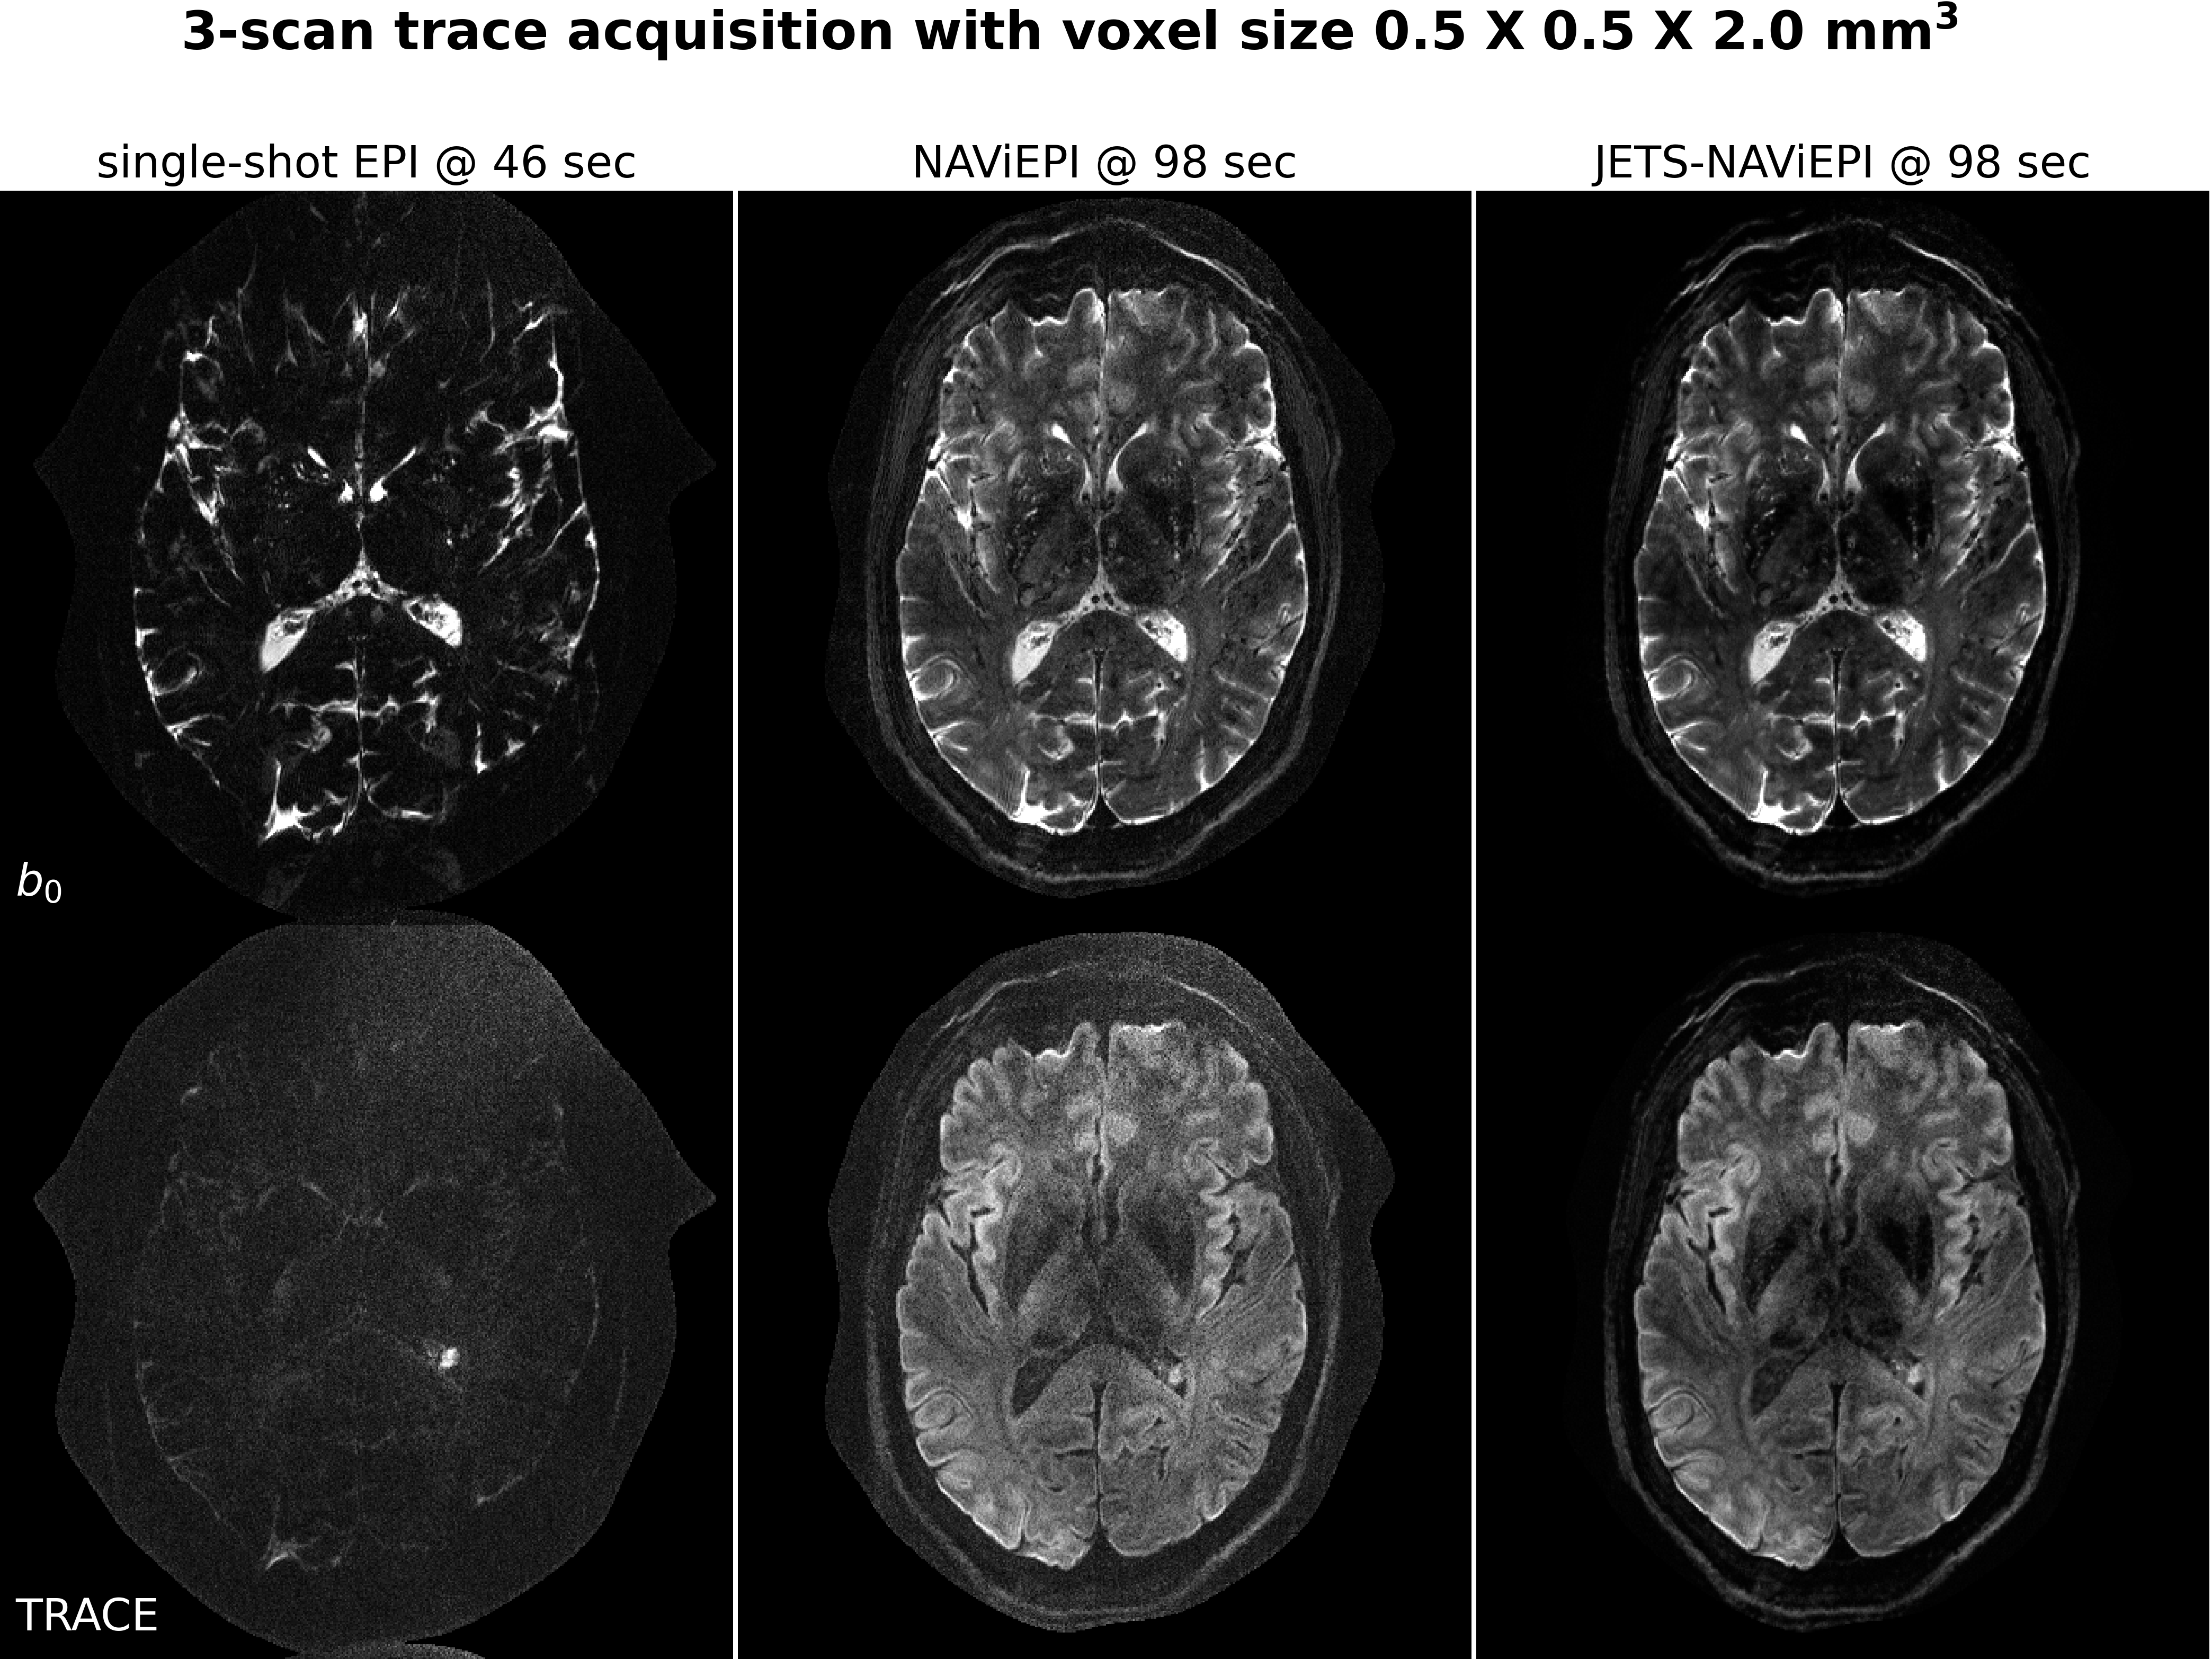
\includegraphics[width=\linewidth]{../figures/graph.png}
        \end{graphicalabstract}

        %%Research highlights
        \begin{highlights}
            \item Navigator-based interleaved EPI acquisition with
            minimal distortion mismatch between echoes

            \item Novel accelerated diffusion acquisition
            with shifted phase encoding among diffusion directions
            for complementary $k$-$q$-space sampling at \SI{7}{\tesla}

            \item Generalized joint $k$-$q$-slice
            diffusion-weighted image reconstruction
            with overlapping locally low-rank regularization

            \item Efficient simultaneous multi-slice (SMS)
            image reconstruction

            \item 3-scan trace acquisition with the voxel size
            $0.5\times0.5\times2.0$~mm$^3$ and 60 slices
            at \SI{1.5}{\minute}
        \end{highlights}

        \begin{keyword}
            %% keywords here, in the form: keyword \sep keyword
            Diffusion-weighted magnetic resonance imaging \sep
            Echo planar imaging \sep
            Navigator \sep
            Ultra-high field \sep
            Joint reconstruction \sep
            Low rank \sep
            Simultaneous multi slice
        \end{keyword}

    \end{frontmatter}

    \pagebreak
    \linenumbers

    % ************************************************************************ %
    \section{Introduction}
    \label{SEC:Intr}

    Diffusion-weighted magnetic resonance imaging (DW-MRI)
    \citep{lebihan_1986_diff,merboldt_1985_diff} is a non-invasive modality
    that is sensitive to the intravoxel Brownian motion of water molecules.
    DW-MRI forms the basis for diffusion tensor imaging (DTI) \citep{basser_1994_dmri,mori_2001_track}
    and high angular resolution diffusion imaging (HARDI) \citep{tuch_2002_hardi},
    and has been widely used in acute brain ischemia diagnosis, in tumor detection and staging,
    and in neuroscience \citep{jones_2010_diff}.

    For DW-MRI acquisition, the commonly used pulse sequence is
    single-shot echo-planar imaging (SS-EPI) \citep{mansfield_1977_epi}.
    SS-EPI is capable of rapidly acquiring one DW image per radio-frequency excitation
    at the order of \SI{100}{\ms}, and is thus motion robust.
    However, conventional SS-EPI,
    even with three-fold accelerated acquisition \citep{bammer_2001_epi_sense}
    using parallel imaging
    \citep{roemer_1990_pi,ra_1993_sense,pruessmann_1999_sense,griswold_2002_grappa},
    still suffers from low spatial resolution and geometric distortions.

    In the quest for high spatial-angular-temporal-resolution
    and minimal-geometry-distortion DW-MRI,
    tremendous efforts have been made.
    Techniques for the correction of image distortions
    induced by off-resonances and eddy currents
    have been developed \citep{andersson_2003_topup}.
    Furthermore, gSlider \citep{setsompop_2018_gslider} with
    blipped-CAIPI \citep{setsompop_2012_blipped}
    for simultaneous multi-slice (SMS)
    \citep{maudsley_1980_sms,breuer_2005_caipi}
    was proposed to achieve high-resolution DW-MRI.
    Advanced pulse sequences based on
    multi-shot EPI have also been developed,
    including but not limited to interleaved EPI (iEPI)
    \citep{butts_1993_iepi},
    PROPELLER \citep{pipe_2002_blade}, and
    readout-segmented EPI (rsEPI)
    \citep{porter_2009_resolve,heidemann_2010_resolve7t}.

    Based on four-shot iEPI,
    multiplexed sensitivity encoding (MUSE) image reconstruction
    achieved DW-MRI with a sub-millimeter in-plane resolution
    and maximal $b$-value \SI{800}{s/mm^2} at \SI{3}{\tesla}
    \citep{chen_2013_muse}.
    The four-shot iEPI employed in MUSE acquired
    an in-plane fully-sampled $k$-space, except partial Fourier.
    Every shot (segment), corresponding to four-fold undersampling,
    was then reconstructed via parallel imaging
    to obtain shot-to-shot phase variation.
    This indicates that increasing the number of shots in MUSE
    will result in higher undersampling per shot,
    and consequently, degrade shot phase estimation \citep{wu_2017_diff}.
    % On the other hand, the use of in-plane fully-sampled four-shot iEPI
    % is challenging at ultra-high field (e.g.~\SI{7}{\tesla}),
    % because the SAR is linearly proportional
    % to the square of the field strength.

    Alternatively, navigator-based iEPI acquisition has been proposed
    \citep{jeong_2013_navims,dai_2017_navi,dai_2018_navi}.
    These proposals allow for a larger number of shots,
    and hence higher spatial resolution.
    However, due to the use of different ESP
    between the imaging echo and the navigator echo,
    these proposals suffered from geometric distortion mismatch
    between the two echoes and thus required specific compensation methods.
    In contrast, rsEPI \citep{porter_2009_resolve,heidemann_2010_resolve7t}
    used the same readout segment for both echoes,
    and thus required no distortion correction of navigator echoes.

    Beyond the MUSE-type parallel imaging reconstruction,
    compressed sensing \citep{lustig_2007_cs,block_2007_cs}
    has been explored.
    For instance, multi-shot reconstruction techniques
    based on structured low-rank matrix completion (MUSSELS)
    \citep{mani_2017_mussels,bilgic_2019_neatr} achieved
    5-shot DW-MRI with 9-fold undersampling per shot.
    Recently, JULEP \citep{dai_2023_julep}
    incorporated explicit phase mapping into MUSSELS.
    These reconstruction techniques, i.e., MUSE, MUSSELS and JULEP,
    targeted the reconstruction of one DW image
    from interleaved EPI acquisition,
    and did not explore joint-$k$-$q$-space undersampling or reconstruction.

    Joint-$k$-$q$-space undersampling can be achieved
    via proper regularization along the diffusion encoding direction.
    Relevant examples are diffusion undersampling
    with Gaussian process estimated reconstruction (DAGER)
    \citep{wu_2019_dager} and
    magnitude-based spatial-angular locally low-rank regularization
    (SPA-LLR) \citep{hu_2020_spa_llr}.
    However, DAGER addressed the reconstruction problem
    of single-shot EPI acquisition and
    SPA-LLR focused on the reconstruction
    of single-band and fully-sampled iEPI acquisition.

    In this work, we propose a Joint $k$-$q$-slice rEconsTruction framework
    for Shift-encoded NAVigator-based interleaved EPI
    at \SI{7}{\tesla} (dubbed JETS-NAViEPI).
    Our pulse sequence, NAViEPI, differs from most existing techniques.
    First, NAViEPI builds upon interleaved EPI, thereby allowing for
    fast and efficient $k$-space coverage.
    Second, inspired by rsEPI, NAViEPI ensures the same effective ESP
    between the imaging and the navigator echo,
    thereby minimizing geometric distortion and
    allowing for the use of a larger number of shots.
    NAViEPI essentially integrates the advantages of both iEPI and rsEPI.
    Third, NAViEPI utilizes undersampled multi-shot iEPI,
    thereby alleviating the SAR problem at \SI{7}{\tesla}.
    Fourth, NAViEPI shifts the $k$-space in-plane sampling pattern
    along the phase encoding ($k_y$) direction.
    This shifting creates complementary $k$-$q$-space sampling,
    which leads to the possibility of
    our joint $k$-$q$-slice reconstruction.
    Specifically, we employ spatial-diffusion overlapping LLR regularization
    to jointly reconstruct all diffusion encodings and multi-band slices.
    In vivo experiments at \SI{7}{\tesla} and
    comparisons with other techniques
    demonstrate the efficiency of our proposed method in
    achieving high spatial resolution DW-MRI at ultra-high field.

    \clearpage

    % ************************************************************************ %
    \section{Materials and methods}
    \label{SEC:Meth}

    \begin{figure}
        \centering
        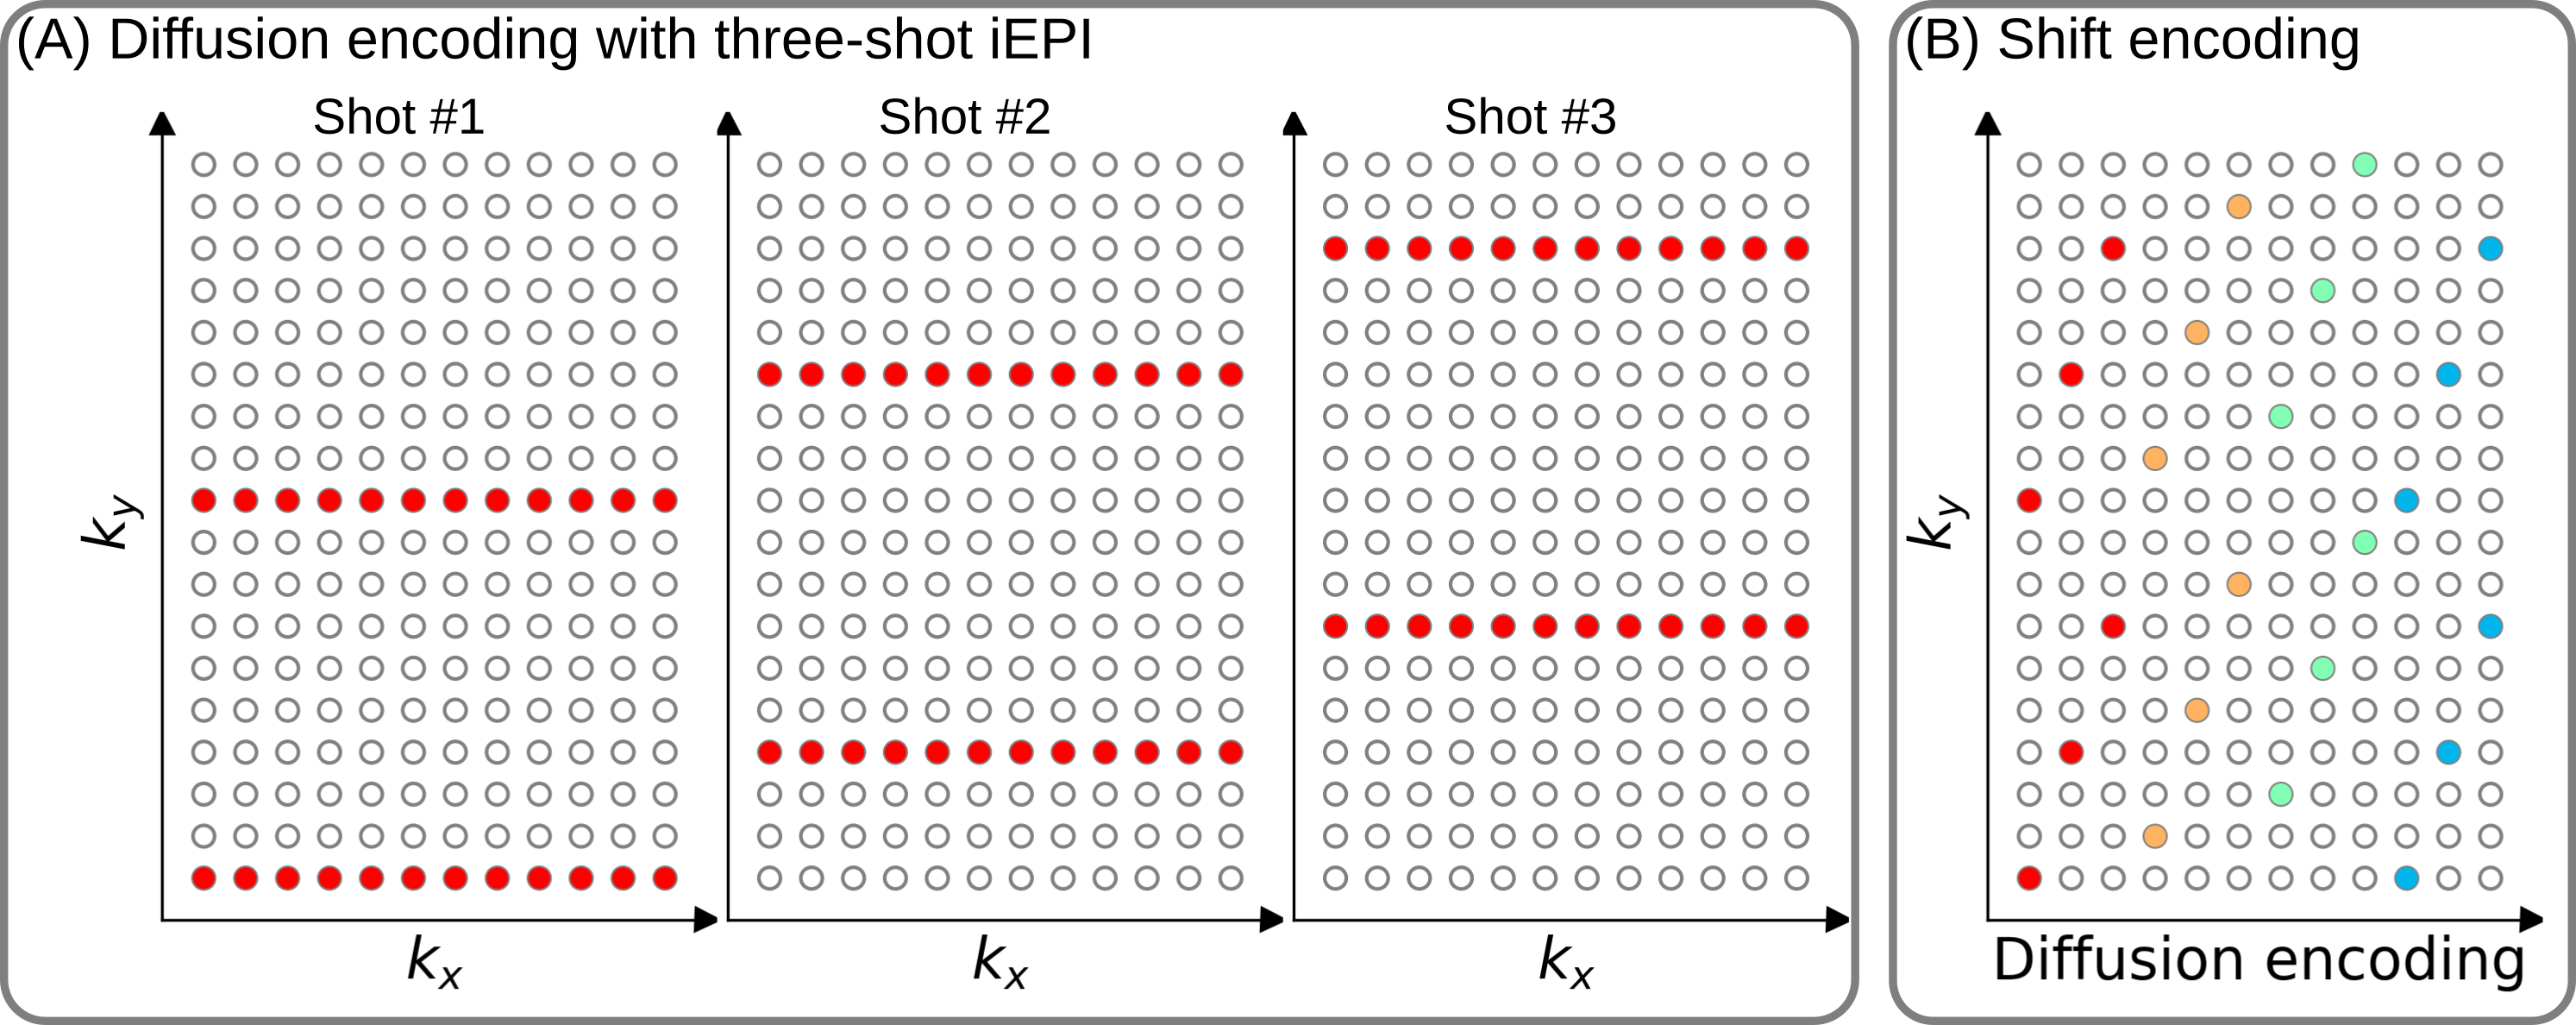
\includegraphics[width=\linewidth]{../figures/fig1.png}
        \caption{(A) An example DW-MRI acquisition
        with three-shot interleaved EPI acquisition.
        (B) The proposed $k_y$ shifted diffusion encoding scheme.
        This example employs three shots per DW image.
        Therefore, every three columns have the same color.}
        \label{FIG:sampling}
    \end{figure}

    % ============================== %
    \subsection{Multi-band shift-encoded iEPI acquisition}

    \cref{FIG:sampling} (A) displays the diffusion-weighted image
    acquisition based on three-shot interleaved EPI
    with three-fold in-plane undersampling.
    Conventionally, such a sampling pattern is repeated
    for all diffusion directions.
    In contrast, we propose the $k_y$-shifted diffusion encoding,
    as shown in \cref{FIG:sampling} (B).
    The interleaved EPI sampling pattern is shifted by one $k_y$ line
    per diffusion direction,
    with the cycling period being the in-plane undersampling factor.

    It is worth noting that, as shown in \cref{FIG:sampling} (A),
    the undersampling factor of one segment is
    $R_\text{in-plane} \times N_\mathrm{shot}$
    (ignore multi-band undersampling here),
    yielding nine-fold in-plane undersampling in this example.
    In other words, the undersampling factor per segment
    linearly scales up with the number of shots.
    Consequently, conventional self-gating reconstruction techniques,
    e.g.~MUSE, suffer from degraded shot-to-shot phase estimation,
    which in turn limits the number of shots and spatial resolution.

    \begin{figure}
        \centering
        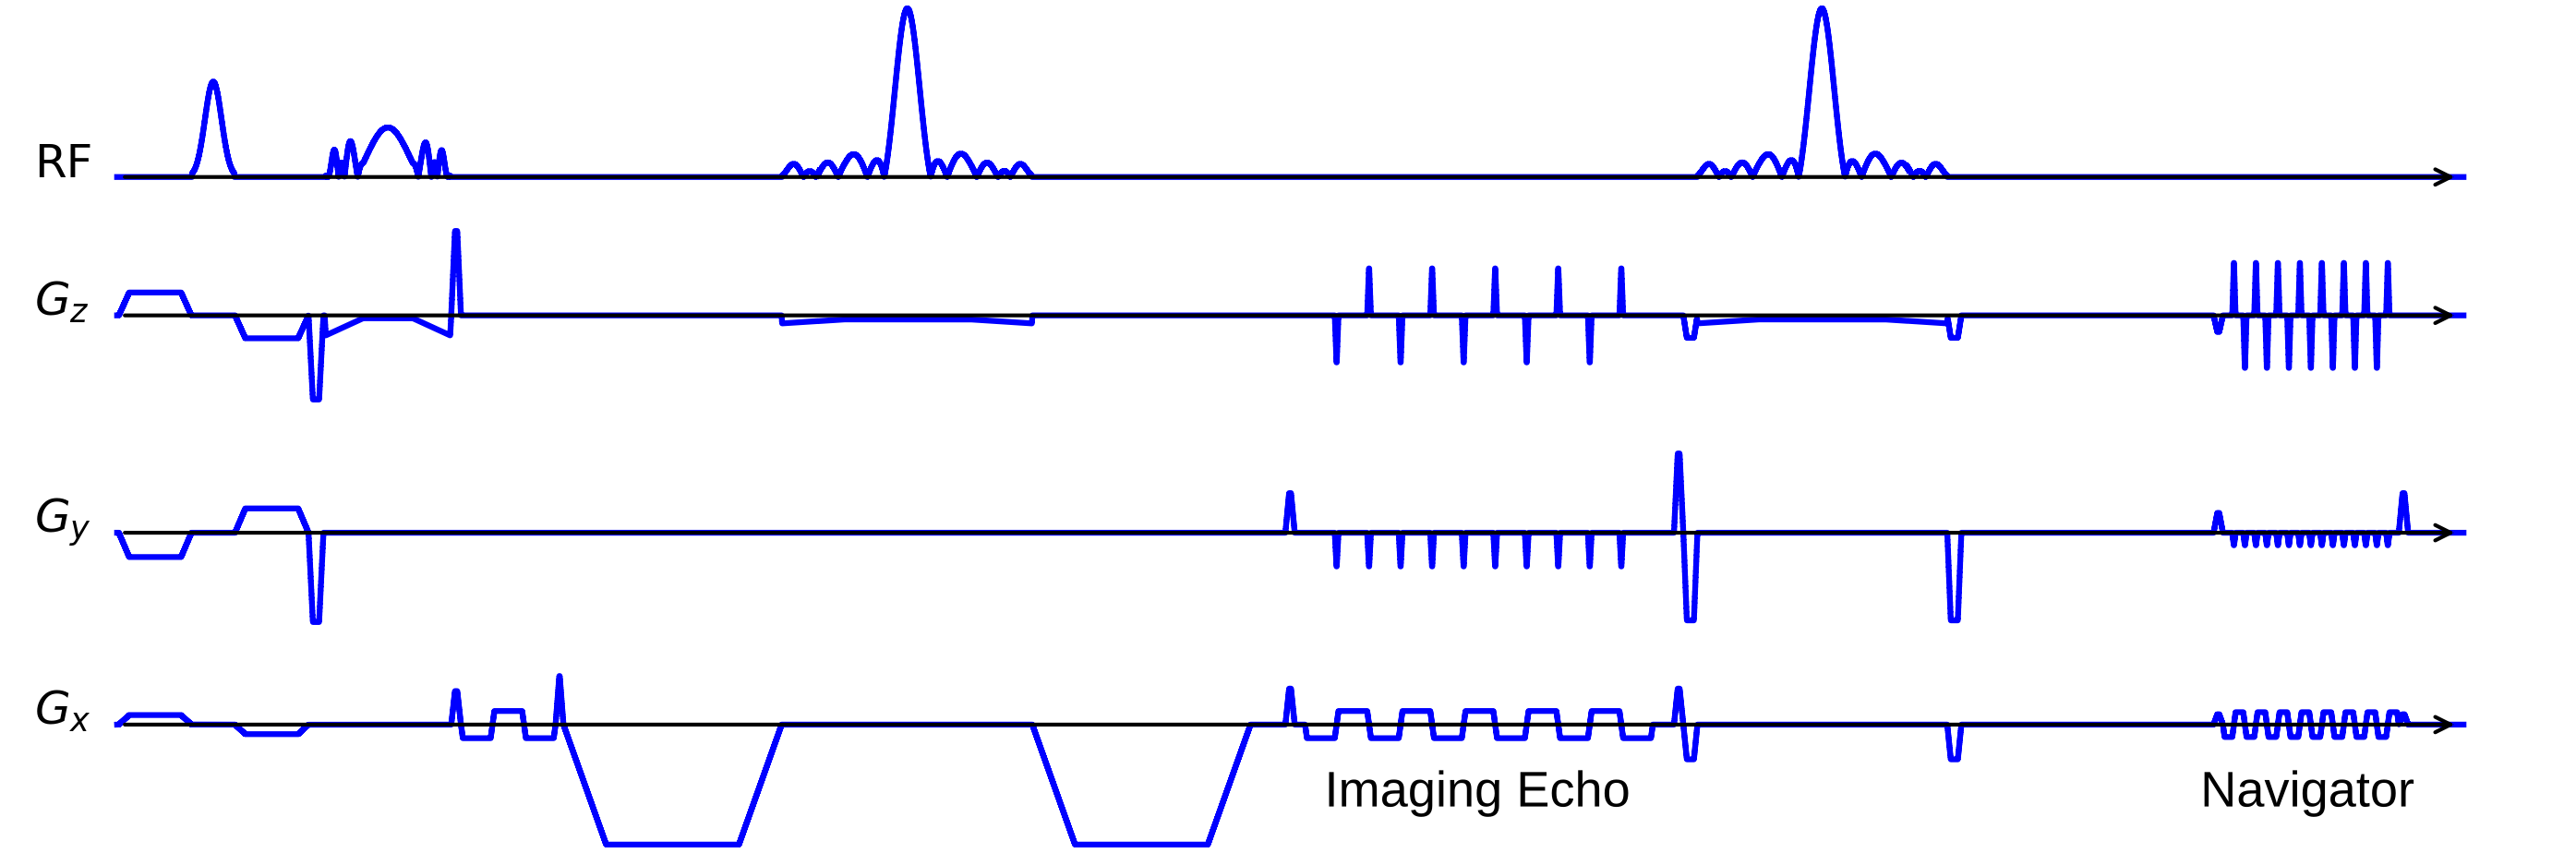
\includegraphics[width=\linewidth]{../figures/fig2.png}
        \caption{The NAViEPI sequence diagram.
        SMS is utilized for the acquisition of both imaging and
        navigator echoes. While the acceleration factor per navigator is
        the same as listed in \cref{TAB:ACQ},
        the acceleration factor per imaging echo is
        in addition linearly scaled by the number of shots.}
        \label{FIG:seq}
    \end{figure}

    \subsection{NAViEPI: Navigator-based iEPI with consistent effective ESP
    between the imaging and the navigator echo - where iEPI meets rsEPI}

    % TODO: \cref sequence figure
    Instead of the self-gated MUSE with in-plane fully-sampled iEPI
    and a limited number of shots,
    We propose NAVigator-based interleaved EPI (NAViEPI),
    as illustrated in \cref{FIG:seq}.
    Inspired by rsEPI \citep{porter_2009_resolve},
    NAViEPI enforces a consistent effective ESP
    between the imaging and the navigator echo,
    thereby minimizing distortion mismatch between the two echoes.

    Since one imaging echo presents
    one segment in multi-shot EPI acquisition,
    its effective ESP is defined as
    \begin{equation}
        \mathrm{ESP}_{\mathrm{eff}} = \frac{\mathrm{ESP}}{R_\text{in-plane} \times N_\mathrm{shot}}
        \label{EQU:Eff_ESP_Imag}
    \end{equation}
    Here, a larger number of shots (segments) increases
    the undersampling factor per segment (see \cref{FIG:sampling}),
    but decreases the effective ESP.
    Since the navigator echo is acquired for each segment,
    its in-plane undersampling factor
    equals $R_\text{in-plane}$.
    Therefore, the effective ESP of the navigator echo
    must match that of the imaging echo,
    as given in \cref{EQU:Eff_ESP_Imag}.
    With a matching effective ESP,
    the base resolution of the navigator echo
    can then be determined.

    % ============================== %
    \subsection{In vivo acquisition protocols}

    We implemented multiple in-vivo acquisition protocols
    at a clinical \SI{7}{\tesla} MR system
    (MAGNETOM Terra, Siemens Healthineers, Erlangen, Germany)
    equipped with a 32-channel head coil (Nova Medical, Wilmington, MA, USA)
    and the XR-gradient system
    (maximum gradient strength \SI{80}{\milli\tesla / \meter}
    with a peak slew rate of \SI{200}{\tesla / \meter / \second}).
    To calibrate coil sensitivity maps, reference scans employed a gradient-echo (GRE) sequence.
    Spectral fat saturation and mono-polar diffusion-encoding gradients were used.
    The phase-encoding direction was selected as anterior-to-posterior.

    \newcolumntype{a}{p{0.36\textwidth}}
    \newcolumntype{b}{p{0.14\textwidth}}
    \begin{threeparttable}
        \centering
        \caption{NAViEPI acquisition protocols}
        \label{TAB:ACQ}
        \begin{tabular}{ a | b b b b }
            \toprule
            \multirow{2}{*}{\textbf{Protocol}} & \multicolumn{2}{c}{$\mathbf{1.0}$~\textbf{mm isotropic}} & \multicolumn{2}{c}{\textbf{sub-millimeter}} \\ \cmidrule(lr){2-3} \cmidrule(lr){4-5}
            & \#1 & \#2 & \#3 & \#4 \\ \hline
            \rowcolor{gray!20} Diffusion mode & \multicolumn{2}{c}{MDDW~\tnote{(1)}} & \multicolumn{2}{c}{3-scan trace} \\
            Diffusion scheme & \multicolumn{4}{c}{monopolar} \\
            \rowcolor{gray!20} Diffusion direction & $20$ & $114$ & \multicolumn{2}{c}{$3$} \\
            $b$-value (\si{s/mm^2}) & $1000$ & 3-shell~\tnote{(2)} & \multicolumn{2}{c}{$1000$} \\
            \rowcolor{gray!20} $b_0$ & $0$ & $12$ & \multicolumn{2}{c}{1} \\
            FOV (\si{\square\mm}) & $200$ & $214$ & \multicolumn{2}{c}{$220$} \\
            \rowcolor{gray!20} In-plane resolution (\si{\square\mm}) & \multicolumn{2}{c}{$1.0$} & \multicolumn{2}{c}{$0.5$} \\
            Slice thickness (\si{\mm}) & \multicolumn{2}{c}{$1.0$} & \multicolumn{2}{c}{$2.0$} \\
            \rowcolor{gray!20} Slices & $141$ & $114$ & \multicolumn{2}{c}{$60$} \\
            Navigator & No & No & Yes & No \\
            \rowcolor{gray!20} Shots & $4$ & $2$ & $5$ & $1$ \\
            TR (\si{ms}) & $7700$ & $5200$ & $4400$ & $8000$ \\
            \rowcolor{gray!20} TEs (\si{ms}) & $67$ & $66$ & $58/95.1$ & $143$ \\
            ESP (\si{ms}) & $1.02$ & $0.81$ & $1.52$ & $1.48$ \\
            \rowcolor{gray!20} Bandwidth (\si{Hz/Pixel}) & $1086$ & $1460$ & \multicolumn{2}{c}{$758$} \\
            Partial Fourier & \multicolumn{4}{c}{$6/8$} \\
            \rowcolor{gray!20} Acceleration~\tnote{(3)} & $1\times3$ & $3\times3$ & \multicolumn{2}{c}{$3\times2$} \\
            TA (\si{\minute})~\tnote{(4)} & $10:42$ & $22:25$ & $1:38$ & $0:46$ \\
            \bottomrule
        \end{tabular}
        \begin{tablenotes}{\footnotesize
        	\item[(1)] MDDW: Multi-direction diffusion weighting;
        	\item[(2)] 3-shell: $20$, $30$, and $64$ directions
            with $b$-values of
            $1000$, $2000$,and \SI{3000}{s/mm^2}, respectively;
            \item[(3)] Acceleration: Both in-plane and slice undersampling can be employed, denoted as ($R_\text{in-plane} \times R_\text{slice}$);
            \item[(4)] TA: Total acquisition time.}
        \end{tablenotes}
    \end{threeparttable}

    % \newcolumntype{a}{p{0.36\textwidth}}
    % \newcolumntype{b}{p{0.14\textwidth}}
    % \begin{threeparttable}
    %     \centering
    %     \caption{NAViEPI acquisition protocols}
    %     \label{TAB:ACQ}
    %     \begin{tabular}{ a | b b b b }
    %         \toprule
    %         \multirow{2}{*}{\textbf{Protocol}} & \multicolumn{2}{c}{$\mathbf{1.0}$~\textbf{mm isotropic}} & \multicolumn{2}{c}{\textbf{sub-millimeter}} \\ \cmidrule(lr){2-3} \cmidrule(lr){4-5}
    %         & \#1 & \#2 & \#3 & \#4 \\ \hline
    %         \rowcolor{gray!20} Diffusion mode & \multicolumn{2}{c}{MDDW~\tnote{1}} & \multicolumn{2}{c}{3-scan trace} \\
    %         Diffusion scheme & \multicolumn{4}{c}{monopolar} \\
    %         \rowcolor{gray!20} Diffusion direction & $20$ & $30$ & \multicolumn{2}{c}{$3$} \\
    %         $b$-value (\si{s/mm^2}) & \multicolumn{4}{c}{1000} \\
    %         \rowcolor{gray!20} $b_0$ & 0 & \multicolumn{3}{c}{1} \\
    %         FOV (\si{\square\mm}) & \multicolumn{2}{c}{$200$} & \multicolumn{2}{c}{$220$} \\
    %         \rowcolor{gray!20} In-plane resolution (\si{\square\mm}) & \multicolumn{2}{c}{$1.0$} & \multicolumn{2}{c}{$0.5$} \\
    %         Slice thickness (\si{\mm}) & \multicolumn{2}{c}{$1.0$} & \multicolumn{2}{c}{$2.0$} \\
    %         \rowcolor{gray!20} Slices & $141$ & $124$ & \multicolumn{2}{c}{$60$} \\
    %         Navigator & No & No & Yes & No \\
    %         \rowcolor{gray!20} Shots & $4$ & $2$ & $5$ & $1$ \\
    %         TR (\si{ms}) & $7700$ & $8500$ & $4400$ & $8000$ \\
    %         \rowcolor{gray!20} TEs (\si{ms}) & $67$ & $56$ & $58/95.1$ & $143$ \\
    %         ESP (\si{ms}) & $1.02$ & $1.06$ & $1.52$ & $1.48$ \\
    %         \rowcolor{gray!20} Bandwidth (\si{Hz/Pixel}) & \multicolumn{2}{c}{$1086$} & \multicolumn{2}{c}{$758$} \\
    %         Partial Fourier & \multicolumn{4}{c}{$6/8$} \\
    %         \rowcolor{gray!20} Acceleration~\tnote{2} & $1\times3$ & $3\times2$ & \multicolumn{2}{c}{$3\times2$} \\
    %         TA (\si{\minute})~\tnote{3} & $10:42$ & $9:12$ & $1:38$ & $0:46$ \\
    %         \bottomrule
    %     \end{tabular}
    %     \begin{tablenotes}{\footnotesize
    %     	\item[1] MDDW: Multi-direction diffusion weighting;
    %         \item[2] Acceleration: Both in-plane and slice undersampling can be employed, denoted as ($R_\text{in-plane} \times R_\text{slice}$);
    %         \item[3] TA: Total acquisition time.}
    %     \end{tablenotes}
    % \end{threeparttable}

    This study was approved by the local ethics committee.
    Three volunteers with informed consent obtained before scanning
    participated in this study.
    Detailed acquisition protocols are listed in \cref{TAB:ACQ}.
    \marginnote{R989.1}
    \hl{In the spirit of reproducible research, another volunteer
    with informed consent was recruited
    for the scan of all acquisition protocols,
    and the results were displayed in Supplementary Information.}


	\subsubsection{20-diffusion-direction acquisition
    at \SI{1}{\milli\meter} isotropic resolution}

	As listed in \cref{TAB:ACQ}, Protocol \#1
	with four-shot iEPI and without in-plane undersampling
	was implemented. This protocol represents the acquisition scheme
	employed in many existing multi-shot reconstruction techniques,
	(e.g., MUSE, SPA-LLR, and JULEP).
	The acquired data from this protocol served as ground truth.
    Different reconstruction methods,
    specifically JETS, MUSE, and JULEP were compared.
    We compared with JULEP instead of MUSSELS,
    because JULEP uses not only structured low-rank constraints
    but also explicit phase mapping.

	We then retrospectively reduced the four-shot data to only one shot
	per diffusion encoding without and with the proposed $k_y$ shifting
    to simulate four-fold in-plane undersampling.
    JETS reconstruction was performed on the fully-sampled data
    and the retrospectively undersampled data
    to validate the proposed $k_y$-shifted acquisition.


    \subsubsection{Three-shell acquisition
    at \SI{1}{\milli\meter} isotropic resolution}

    Protocol \#2 in \cref{TAB:ACQ} was implemented
    for multi-shell diffusion tensor imaging (DTI)
    \citep{basser_1994_dmri}.
    We acquired a total of 114 diffusion directions,
    whereas $b_0$ measurements were interspersed
    every ten diffusion directions.
    This protocol was used to demonstrate
    the capability of of JETS in achieving high
    spatial-angular-temporal resolution.


    \subsubsection{3-scan trace acquisition at $0.5\times0.5\times2.0$~\si{\cubic\milli\meter} voxel size}

    As listed in \cref{TAB:ACQ},
    Protocol \#3 was implemented based on
    NAViEPI with five shots per diffusion encoding.
    This protocol was compared against single-shot EPI (Protocol \#4)
    with the same spatial resolution and acceleration,
    such as to demonstrate the sampling efficiency of NAViEPI.


    % ============================== %
    \subsection{Forward modeling}
    Our proposed acquisition method yields
    multi-dimensional multi-band
    $k$-space data $\mathbf{y}_{c,q,s}$,
    where $c$, $q$, $s$ denotes the index of the coil sensitivity map,
    the diffusion encoding, and the shot, respectively.
    Acquisition modeling needs to consider several aspects.

    First, the acquired $k$-space data $\mathbf{y}$ is mapped from
    individual shot images $\mathbf{x}_{q,s,z}$ via the forward model,

    \begin{align}
        \mathbf{y}_{c,q,s} &= \mathbf{P}_{q,s} \mathbf{\Sigma} \mathbf{\Theta}_{z} \mathbf{F} \mathbf{S}_c \mathbf{x}_{q,s,z} \nonumber \\
        \mathbf{y} &\coloneqq \mathbf{E}_1 \mathbf{x} \label{EQU:model_shot}
    \end{align}
    Here, the encoding matrix $\mathbf{E}_1$ comprises
    a chain of linear operators.
    Every shot image $\mathbf{x}$ is point-wise multiplied
    by a set of coil sensitivity maps ($\mathbf{S}$) and Fourier transformed ($\mathbf{F}$).
    The output is then point-wise multiplied by the multi-slice phase map ($\mathbf{\Theta}$)
    with $z$ the slice index in simultaneously excited slices.
    This operator shifts individual slice
    along the phase-encoding direction
    via varying phase modulation \citep{breuer_2005_caipi}.
    The SMS $k$-space data is then
    summed (collapsed, $\mathbf{\Sigma}$) along the slice dimension and
    masked (point-wise multiplied, $\mathbf{P}$) by
    the sampling pattern of each diffusion encoding and shot.

    % The SMS modeling in \cref{EQU:model_shot} directly encodes
    % the SMS phase shift into the forward model
    % and reflects how the pulse sequence is programmed.
    % Therefore, this physics-driven model differs from
    % other existing methods, e.g.,NEATR
    % NEATR  and JULEP

    Second, for diffusion MRI based on multi-shot EPI,
    multiple shots acquired for a given diffusion encoding
    need to be combined as one DW image ($\mathbf{\tilde{x}}$).
    One possibility is to perform magnitude average
    \citep{chen_2013_muse}
    or root-sum-squares (RSS) \citep{mani_2017_mussels}
    of shot images.
    This method is robust to in-plane motion,
    but sub-optimal concerning SNR
    \citep{guhaniyogi_2016_amuse}.
    Alternatively, shot combination can be done
    via shot-to-shot phase variation correction
    \citep{liu_2005_moco_diff,chen_2013_muse}.
    This can be incorporated into our formulation
    as point-wise multiplication
    between the shot-to-shot phase variation ($\mathbf{\Phi}$) and
    the DW image ($\mathbf{\tilde{x}}$),
    \begin{equation}
         \mathbf{x}_{q,s,z} = \mathbf{\Phi}_{q,s,z} \mathbf{\tilde{x}}_{q,z}
    \end{equation}
    Note that $\mathbf{\tilde{x}}$ can be obtained
    by applying the adjoint of $\mathbf{\Phi}$ to $\mathbf{x}$.
    In MUSE, $\mathbf{\Phi}$ is obtained by parallel imaging reconstruction of all shots
    with subsequent phase smoothing of every shot image.
    Based on this phase correction, the complete forward model follows
    \begin{equation}
        \mathbf{y} \coloneqq \mathbf{E}_2 \mathbf{\tilde{x}} = \mathbf{E}_1 \mathbf{\Phi} \mathbf{\tilde{x}}
        \label{EQU:model_dwi}
    \end{equation}
    where the encoding matrix $\mathbf{E}_2$ comprises the chain of
    the shot-to-shot phase variation $\mathbf{\Phi}$ and
    the encoding matrix $\mathbf{E}_1$.
    We implemented these two encoding operators
    in SigPy \citep{ong_2019_sigpy}.


    % ============================== %
    \subsection{Joint $k$-$q$-slice reconstruction}
    \label{SUBSEC:JETS}

    % TODO: iterative phase smoothing
    Based on the generalized forward models in \cref{EQU:model_shot,EQU:model_dwi},
    our proposed joint $k$-$q$-slice reconstruction can be formulated as a three-step approach.

    \begin{enumerate}[I.]
        \item \textbf{Navigator echo reconstruction}.
        The acquisition of navigator echoes follows the forward model
        in \cref{EQU:model_shot}, so the reconstruction of navigator echoes
        can be formulated as:
        \begin{equation}
            \mathrm{argmin}_\mathbf{x} \left\| \mathbf{y} - \mathbf{E}_1 \mathbf{x} \right\|_2^2
            + \lambda \mathbf{R}(\mathbf{x})
            \label{EQU:solve_navi}
        \end{equation}
    	where $\mathbf{R}(\mathbf{x})$ denotes the regularization functional
    	with the regularization strength $\lambda$.
    	In this work, $\ell^2$ regularization was used,
    	i.e.,~$\mathbf{R}(\mathbf{x}) = \left\lVert \mathbf{x} \right\rVert_2^2$.
        In the case of self-navigating
        (i.e., no navigator acquired) as Protocol \#2,
        the central $k$-space region (i.e., $1/4$ of the full image matrix)
        of each segment is used as $\mathbf{y}$ in \cref{EQU:solve_navi}.


        \item \textbf{Iterative phase smoothing}.
        Shot-to-shot phase variation was extracted from
        the reconstructed navigator echo phases.
        Assuming that phase images are spatially smooth
        \citep{chen_2013_muse,dai_2023_julep},
        \marginnote{R990.12}
        \hl{we employed the adaptive Hanning filter to smooth shot phases,}
        \begin{equation}
        	\mathbf{x} = \mathbf{F}^{-1} \mathcal{H}^K \mathbf{F} \mathbf{x}
        	\label{EQU:ITER_PHASE}
        \end{equation}
    	\hl{where \mbox{$x$} is the reconstructed navigator image from Step I.
    	\mbox{$\mathcal{H}$} is the Hanning window
        with the non-negative integer $K$.
        \mbox{$K$} controls the width of the Hanning window.}

        \item \textbf{Shot-combined reconstruction}.
        Joint reconstruction of all DW images using
        the shot-combined forward model $\mathbf{E}_2$
        with shot-to-shot phase variation from Step II reads:
        \begin{equation}
            \mathrm{argmin}_\mathbf{\tilde{x}} \left\| \mathbf{y} - \mathbf{E}_2 \mathbf{\tilde{x}} \right\|_2^2
            + \lambda \left\| \mathbf{T} ( \mathbf{\tilde{x}} ) \right\|_*
            \label{EQU:solve_dwi}
        \end{equation}
    	Here, LLR regularization was employed in the local spatial-diffusion matrices,
    	based on the theory of partially separable functions
    	\citep{liang_2007_psf,trzasko_2011_lr,zhang_2015_llr}.
    	$\mathbf{T}$ represents a linear operator that
        firstly slides a local patch window
    	through all DW images and then
    	flattens every set of local patches
    	to construct two-dimensional (2D) spatial-diffusion matrices.
        The spatial dimension equals the block size,
        and the diffusion dimension is the number of diffusion encodings.
        $\left\| \mathbf{T} ( \mathbf{\tilde{x}} ) \right\|_*$
        is the nuclear norm, i.e.~the sum of singular values
        of a spatial-diffusion matrix.
    	This nuclear norm regularization was accomplished via
    	singular value thresholding (SVT) of each spatial-diffusion matrix
        \citep{cai_2010_svt}.
        After SVT, the adjoint of $\mathbf{T}$, $\mathbf{T}^H$,
        was needed to reorder
        pixel values from the spatial-diffusion matrices
        back to DW images.
        To alleviate checkerboard artifacts induced
        by LLR regularization with non-overlapping blocks
        \citep{hu_2020_spa_llr},
        we employed overlapping blocks.
        In this case, values from overlapping positions are summed up
        to the output of $\mathbf{T}^H$.
        To enable the correct use of $\mathbf{T}^H$,
        we element-wise divided the output of $\mathbf{T}^H$
        by a scaling matrix. This matrix was obtained via
        $\mathbf{T}^H (\mathbf{T}(\mathbf{1}))$,
        where $\mathbf{1}$ denotes the matrix of all ones
    	with the same shape as the input $\mathbf{x}$.

    \end{enumerate}

    % ============================== %
    \subsection{Reconstruction}

    The acquired raw data was read in by twixtools
    (\url{https://github.com/pehses/twixtools}).
    Ramp-sampling regridding and FOV/2-ghost correction were also performed in twixtools.
    Subsequently, coil sensitivity maps were computed from reference scans
    using ESPIRiT \citep{uecker_2014_espirit} in SigPy \citep{ong_2019_sigpy}.

    With this pre-processing as well as
    the implemented forward models and proximal operator,
    the inverse problem in \cref{EQU:solve_dwi} was solved by
    the alternating direction method of multipliers (ADMM) \citep{boyd_2010_admm}.

    ADMM solves the minimization problems in an alternating update scheme,
    \begin{equation}
        \left\{\begin{matrix}
            \begin{aligned}
                \mathbf{x}^{(k+1)} &:= \argmin_{\mathbf{x}} \norm{\mathbf{y} - \mathbf{E}(\mathbf{x})}^2 + \rho/2 \norm{\mathbf{T}\mathbf{x} - \mathbf{z}^{(k)} + \mathbf{u}^{(k)}}_2^2 \\
                \mathbf{z}^{(k+1)} &:= \mathcal{T}_{\lambda/\rho} (\mathbf{T} \mathbf{x}^{(k+1)} + \mathbf{u}^{(k)}) \\
                \mathbf{u}^{(k+1)} &:= \mathbf{u}^{(k)} + \mathbf{T} \mathbf{x}^{(k+1)} - \mathbf{z}^{(k+1)}
            \end{aligned}
        \end{matrix}\right.
        \label{EQU:ADMM}
    \end{equation}
    where $k$ denotes the ADMM iteration.
    $\mathbf{z}$ is the auxiliary variable ($\mathbf{z} = \mathbf{T}\mathbf{x}$),
    and $\textbf{u}$ is the Lagrangian multipliers.
    Importantly, when solving \cref{EQU:model_shot},
    $\textbf{x}$ denotes shot images and $\mathbf{E}$ denotes $\mathbf{E}_1$ in \cref{EQU:ADMM}.
    In contrast, $\textbf{x}$ denotes shot-combined images and $\mathbf{E}$ denotes $\mathbf{E}_2$
    when solving \cref{EQU:model_dwi}.
    $\mathbf{x}$ can be solved using linear least square algorithms,
    e.g.~conjugate gradients \citep{hestenes_1952_cg},
    while $\mathbf{z}$ is updated via singular value thresholding
    ($\mathcal{T}$) with the thresholding parameter $\lambda / \rho$.
    The coupling parameter $\rho$ is effective in both the update of $\mathbf{x}$ and $\mathbf{z}$.
    It acts as Tikhonov regularization strength when updating $\mathbf{x}$,
    but also inversely scales the thresholding strength when updating $\mathbf{z}$.

    In this work, 15 ADMM iterations with $\rho = 0.05$
    and $\lambda = 0.08$ were used.
    All reconstructions were done on a single A100 SXM4/NVLink GPU
    with \SI{40}{GB} memory (NVIDIA, Santa Clara, CA, USA).

    We compared our proposed joint reconstruction
    with established multi-shot reconstruction techniques,
    specifically, MUSE \citep{chen_2013_muse}
    and JULEP \citep{dai_2023_julep},
    hosted on GitHub by Dr.~Dai \citep{dai_2023_julep}.
    Further, we performed
    the local-PCA denoising \citep{cordero_2019_cplxdwi}
    as implemented in MRtrix \citep{Tournier_2019_mrtrix}
    on the MUSE reconstructed complex DW images.

    The in vivo data acquired from Protocol \#2 in \cref{TAB:ACQ}
    consisted of 126 diffusion directions,
    which exceeds the available GPU memory.
    Therefore, the 126 data volumes were uniformly split
    into three parts for our JETS reconstruction
    with a LLR block width of 6 and the LLR regularization
    in both Steps I and III in \cref{SUBSEC:JETS}.
    In addition, MUSE reconstruction was also performed,
    followed by the local-PCA denoising.
    Reconstructed DWIs were then processed
    by DiPy \citep{garyfallidis_2014_dipy}
    to obtain color-coded fractional anisotropy (cFA) maps.

    \pagebreak

    % ************************************************************************ %
    \section{Results}
    \label{SEC_Resl}

    \begin{figure}
        \centering
        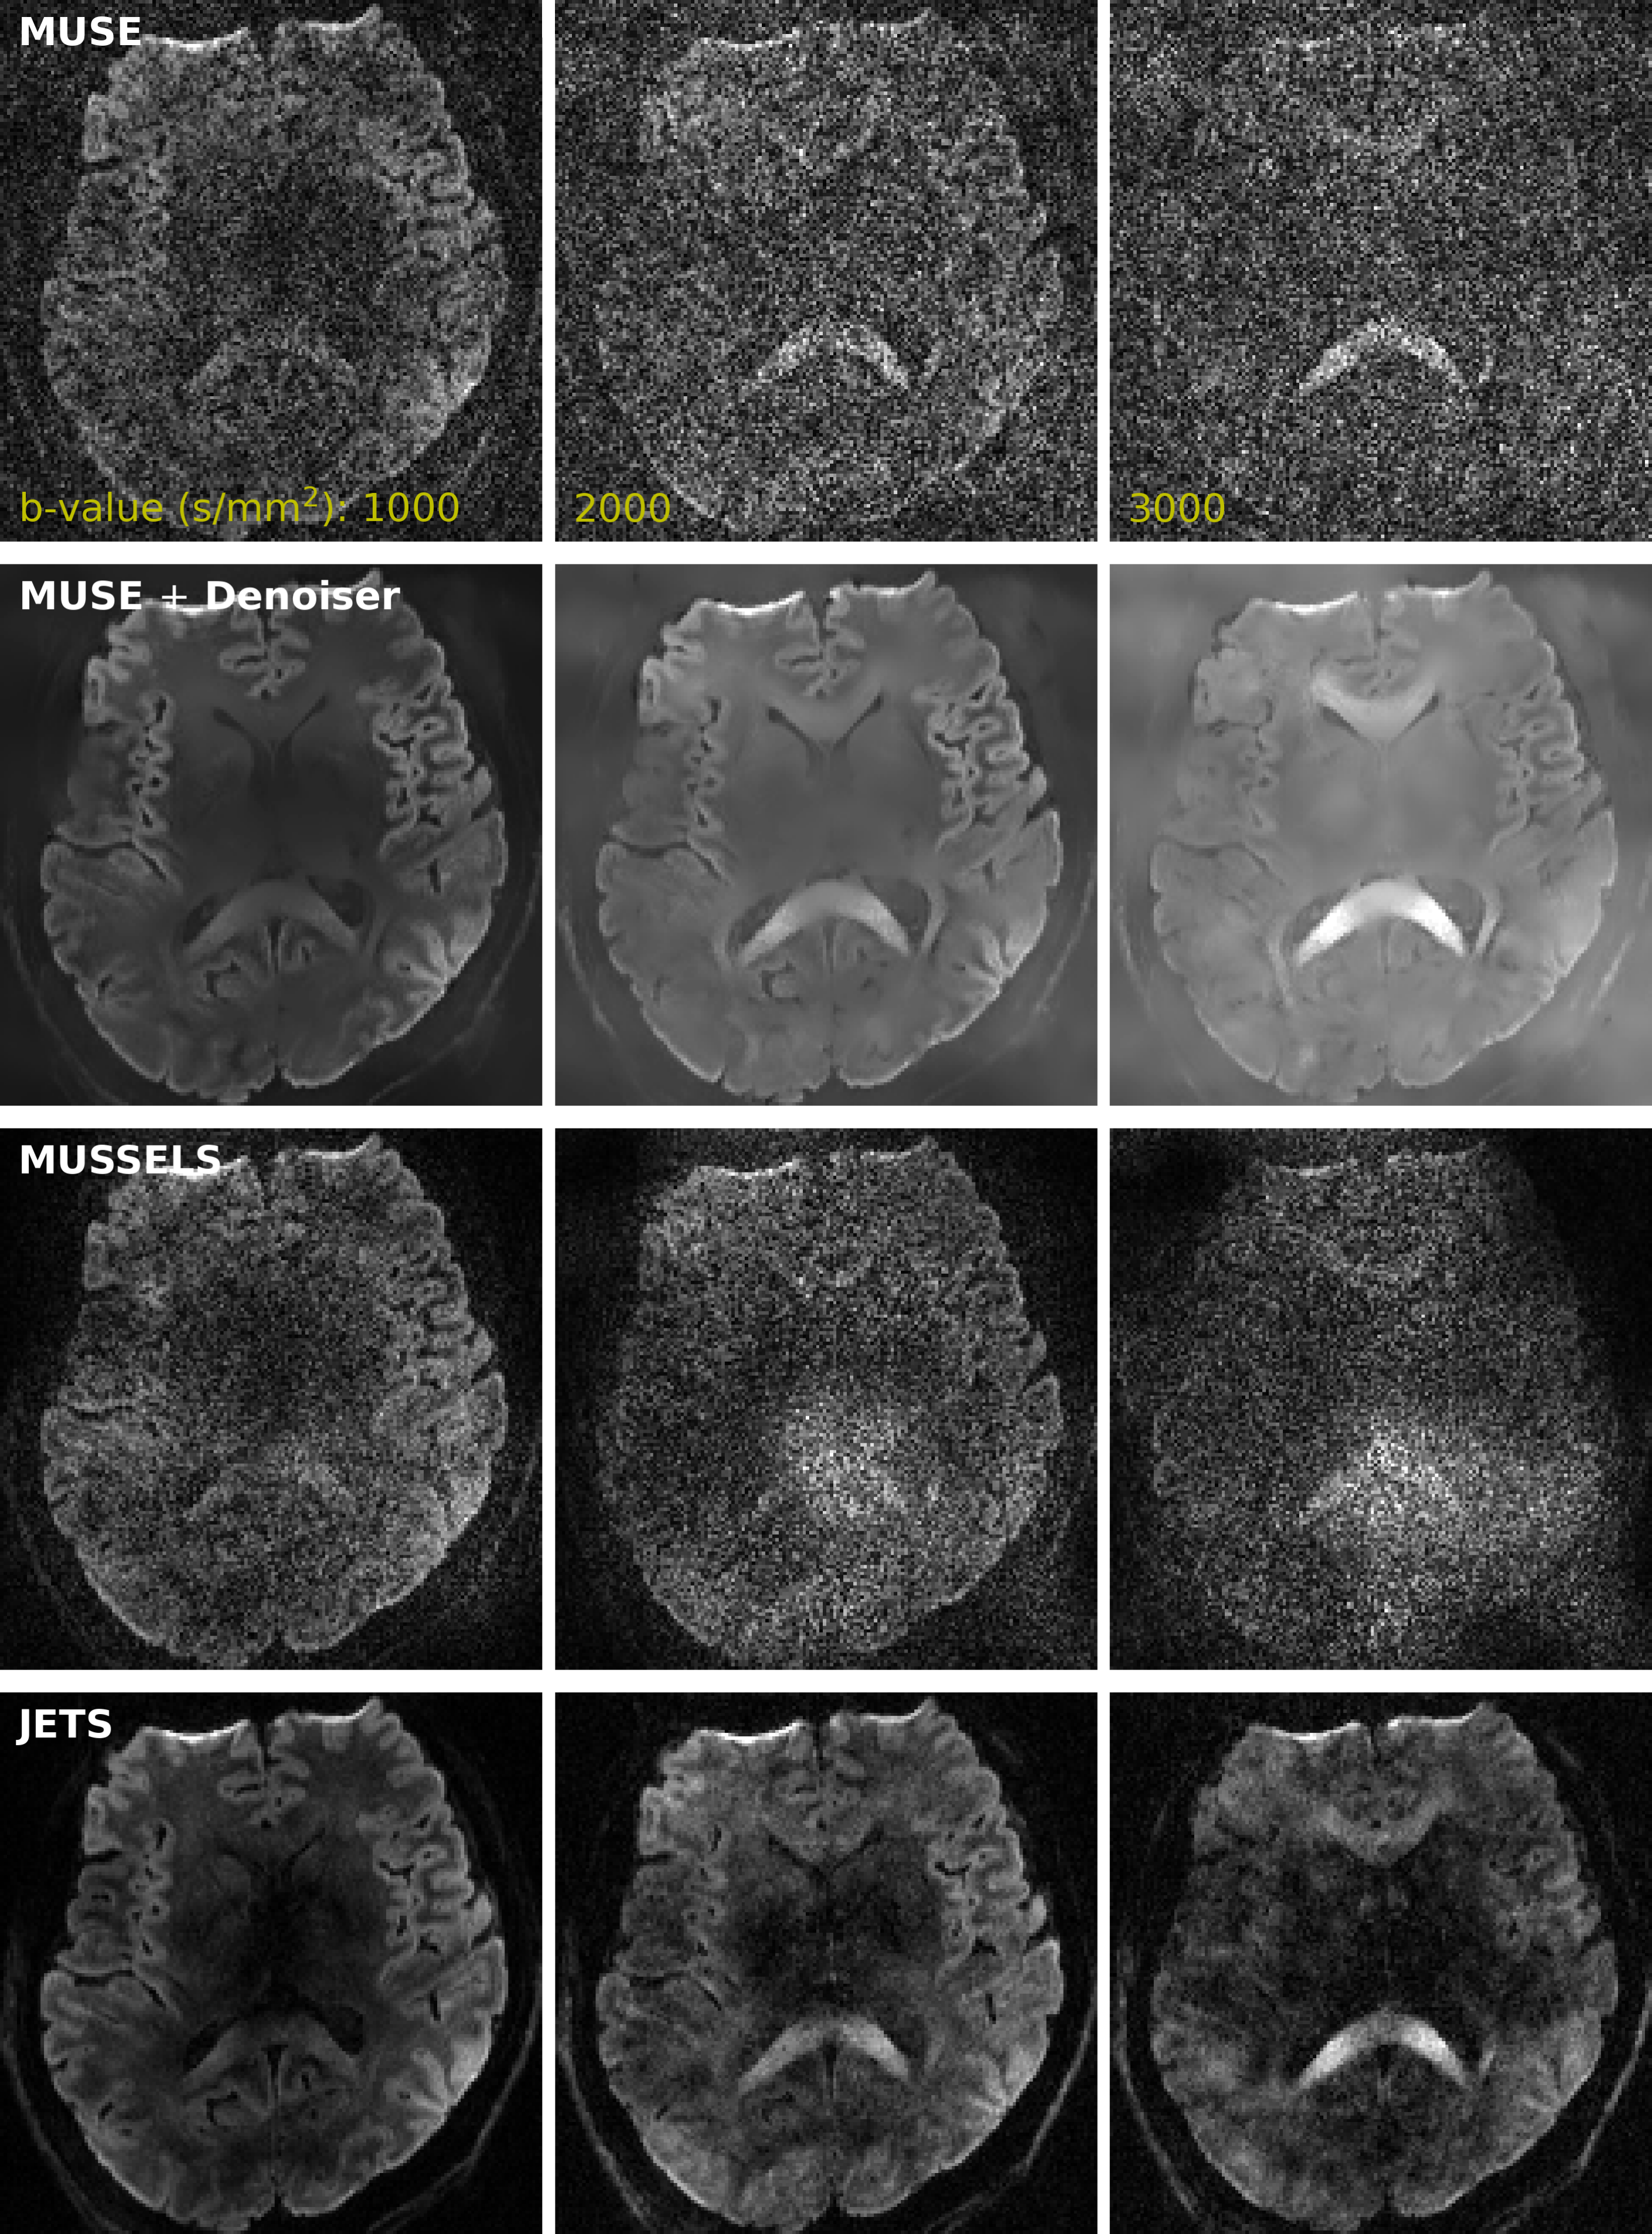
\includegraphics[width=\textwidth]{../figures/fig3.png}
        \caption{Smoothing of shot-to-shot phase variation
        according to \cref{EQU:ITER_PHASE}.
        Navigators from Protocol \#3 were reconstructed
        based on Step I in \cref{SUBSEC:JETS}
        and then used as the input (the column with $K = 0$).}
        \label{FIG:iter_phase}
    \end{figure}

    % ========= %
    \subsection{Smoothing of shot-to-shot phase variation}

    Navigators were acquired with the acceleration rate
    as listed in \cref{TAB:ACQ}.
    Besides, the base resolution of navigators
    (e.g.~32 in Protocol \#3 in \cref{TAB:ACQ})
    was smaller than imaging echoes.
    As a result, reconstructed navigator phases
    (refer to the first column in \cref{FIG:iter_phase})
    from Step I in \cref{SUBSEC:JETS}
    are not spatially smooth.
    Such phases, when used in the shot-combined reconstruction,
    result in signal void artifacts in DW images.
    To address this problem, we utilized the phase smoothing procedure.
    As shown in \cref{FIG:iter_phase},
    \marginnote{R990.12}
    \hl{the ripple-like phase artifact disappears at $K = 5$,
    while retaining the shot-to-shot phase variation.
    In contrast, a larger $K$ (e.g., $K = 20$) makes the filter too strong
    and even partially removes phase variation.}

    \begin{figure}
        \centering
        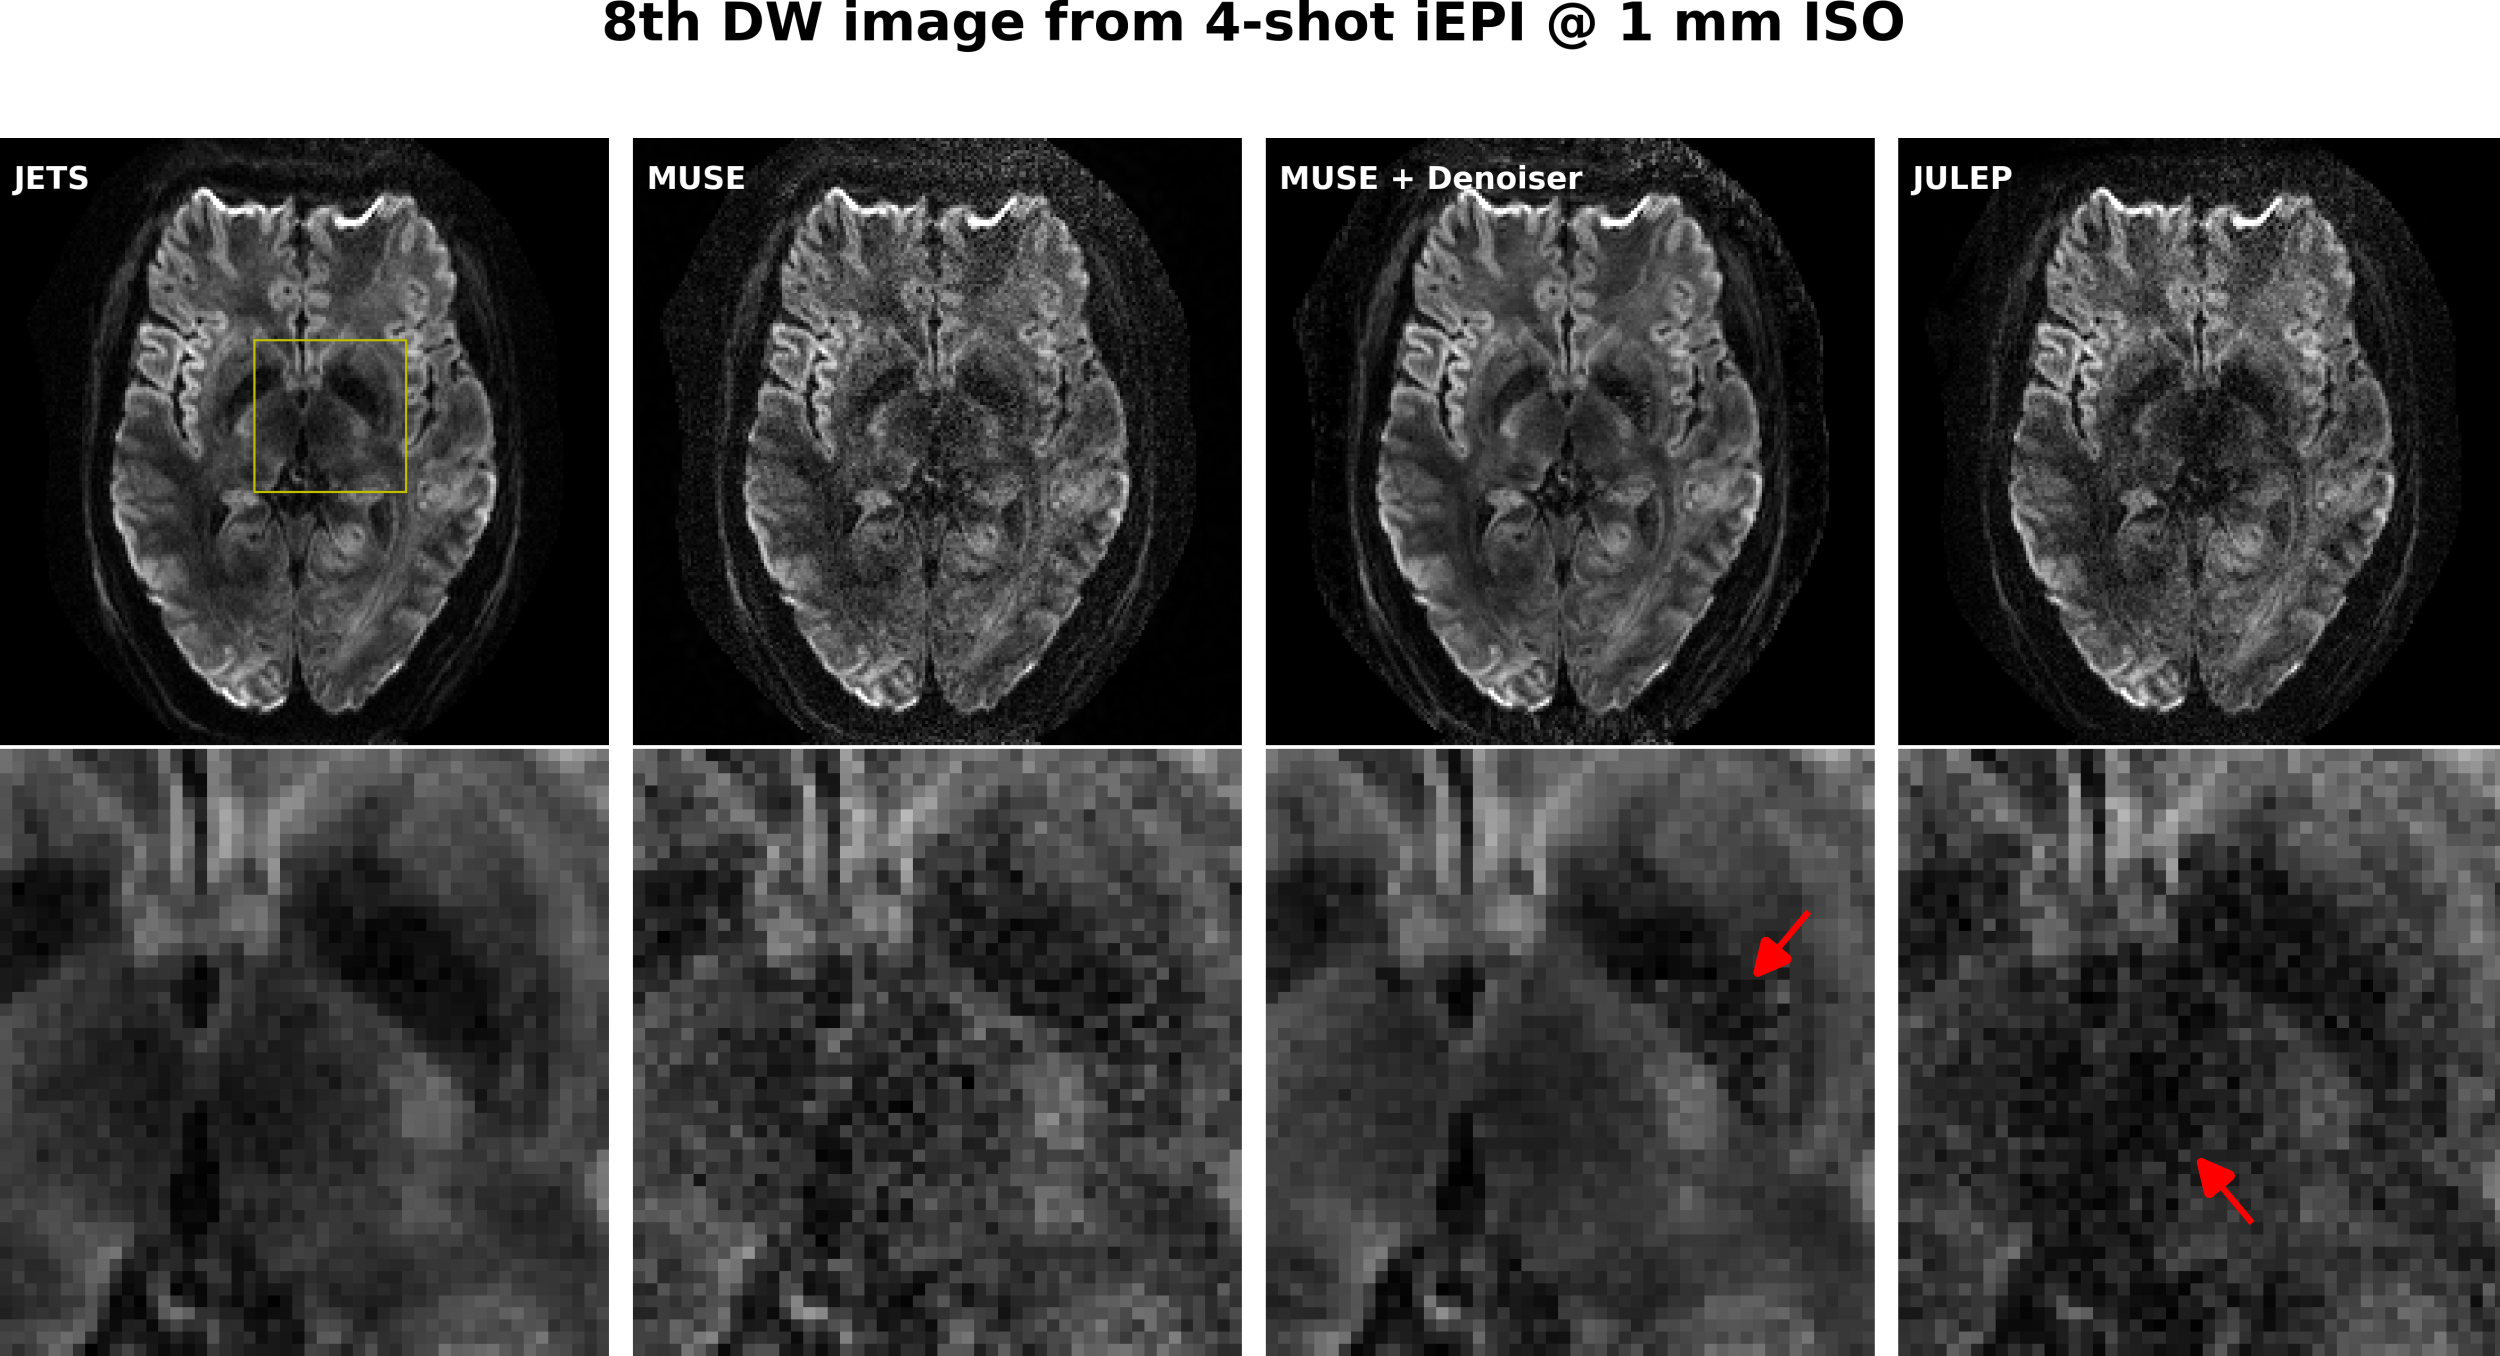
\includegraphics[width=\textwidth]{../figures/fig4.png}
        \caption{Reconstructed DW images
        (the 8th diffusion encoding)
        based on 4-shot iEPI acquisition with 1~mm isotropic resolution
        (Protocol \#1 in \cref{TAB:ACQ}).
        Four reconstruction methods are compared (from left to right):
        JETS, MUSE, MUSE with denoiser, and JULEP.
        The 2nd row displays the magnified views of the yellow square.
        The image from the denoiser (3rd column)
        shows residual noise patterns
        within the globus pallidus (indicated by the red arrow).
        The JULEP reconstruction (4th column) shows signal dropout
        in the central region (indicated by the red arrow).}
        \label{FIG:4shot_comp}
    \end{figure}

    % ========= %
    \subsection{Comparison to MUSE and JULEP with four-shot iEPI acquisition}

    The iterative phase smoothing was also applicable to
    MUSE-type self-navigating reconstruction,
    where shot phases were
    reconstructed from imaging echoes.
    \cref{FIG:4shot_comp} compares our proposed JETS with
    MUSE \citep{chen_2013_muse},
    MUSE with complex-valued local-PCA denoiser
    \citep{cordero_2019_cplxdwi},
    and JULEP \citep{dai_2023_julep}.
    The residual noise from MUSE can be largely removed
    by the denoiser. However, when compared to JETS,
    the denoiser shows residual noise patterns within
    the globus pallidus (indicated by the red arrow).
    JETS also shows better denoising than JULEP.
    The reason is that JETS enforces spatial-diffusion regularization,
    whereas JULEP formulates structured low-rank regularization
    of the four shots for one diffusion encoding.


    \begin{figure}
        \centering
        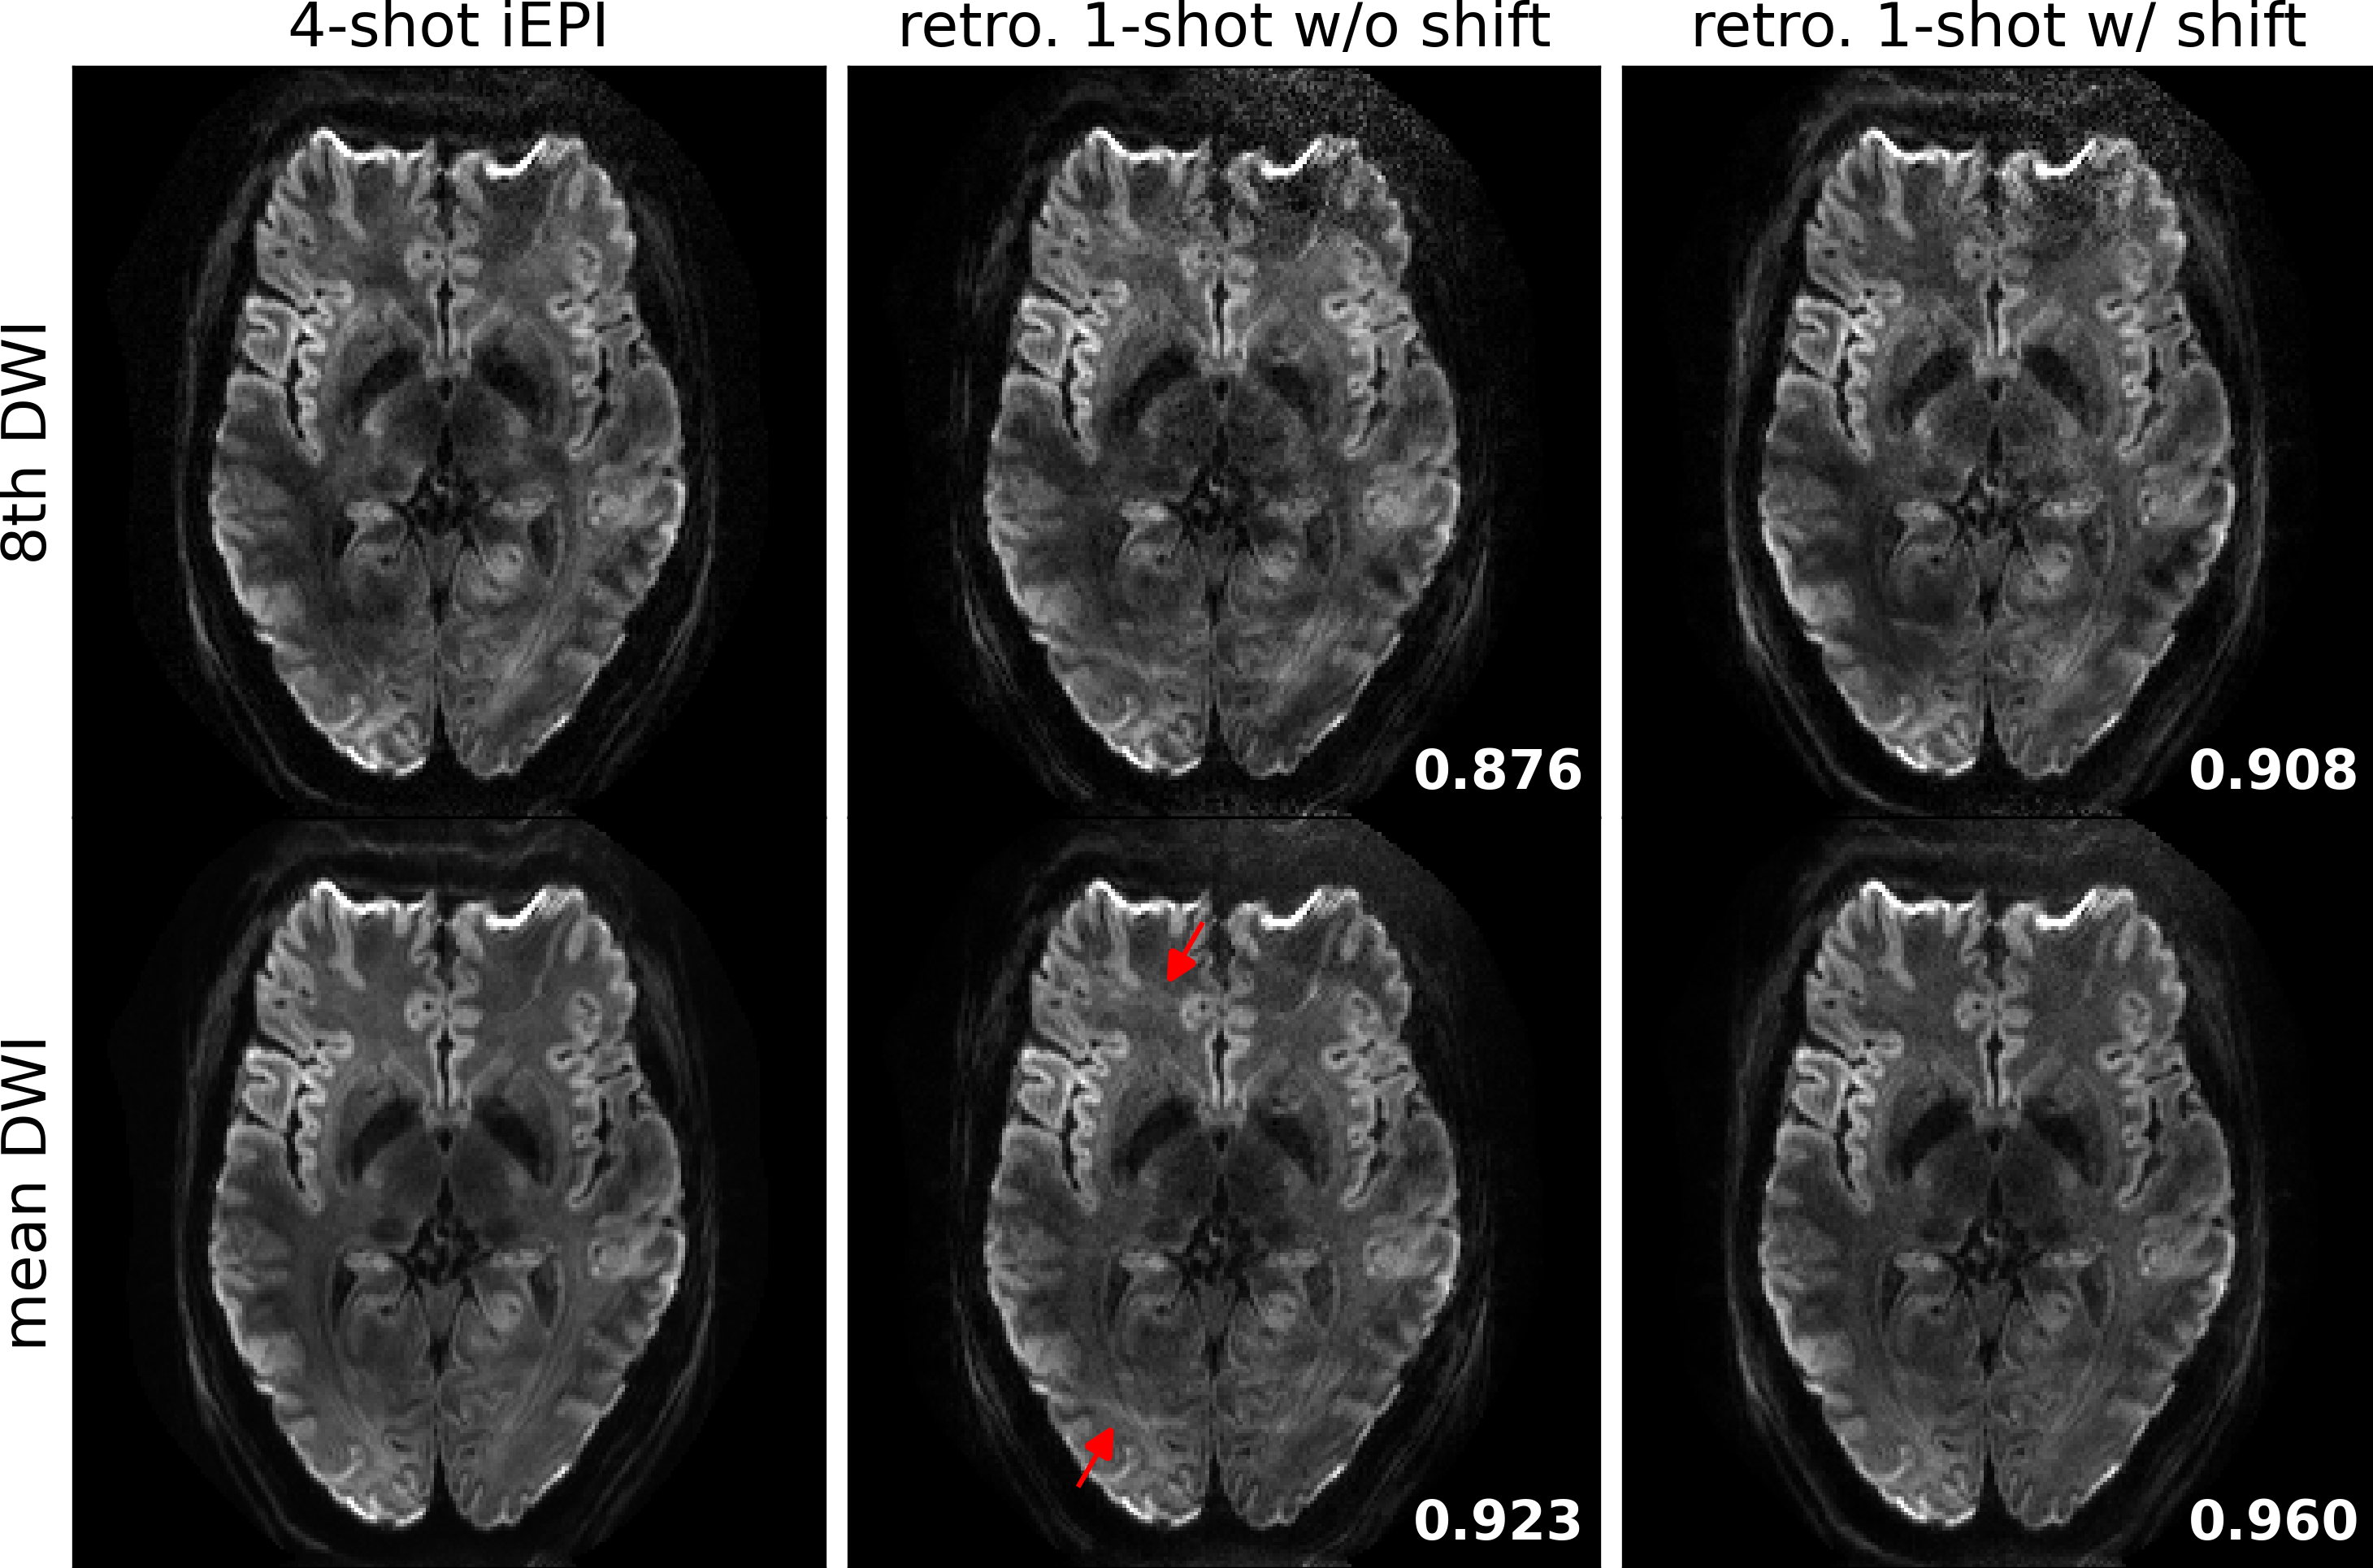
\includegraphics[width=\textwidth]{../figures/fig5.png}
        \caption{Quantitative validation of the proposed
        $k_y$-shift enoding sampling pattern
        based on 4-shot iEPI acquisition with 1~mm isotropic resolution
        (Protocol \#1 in \cref{TAB:ACQ}).
        (Top) the 8th diffusion encoding and
        (bottom) mean DWI over 20 diffusion encodings.
        (1st column) JETS reconstruction of 4-shot iEPI acquisition
        is used as the ground truth.
        The 2nd and the 3rd column displays JETS reconstruction
        of retrospectively undersampled
        1-shot acquisition without and with $k_y$ shifting,
        respectively.
        Residual aliasing artifacts are visible in the reconstruction
        without $k_y$ shifting, as indicated by the red arrows.
        Structural similarity (SSIM) values are computed and
        displayed in the bottom right corners.}
        \label{FIG:retro}
    \end{figure}

    % ========= %
    \subsection{Retrospectively undersampling from the four-shot iEPI acquisition}

    JETS reconstruction results on
    the four-shot prospectively fully-sampled data
    from Protocol \#1 in \cref{TAB:ACQ},
    as well as on the retrospectively undersampled one-shot data
    without and with the proposed $k_y$ shift
    are displayed in \cref{FIG:retro}.
    Residual aliasing artifacts are visible in the reconstruction
    without $k_y$ shifting, as indicated by the red arrows.
    In contrast, the $k_y$ shifting scheme supplies a complementary
    $k$-$q$-space sampling pattern,
    which is beneficial for joint reconstructions such as JETS.
    As shown in \cref{FIG:retro}, JETS results in
    improved SSIM values and reduced aliasing artifacts,
    when compared to the reconstruction without $k_y$ shifting.
    \marginnote{R990.7}
    \hl{\mbox{\cref{FIG:4shot_comp,FIG:retro}} show a slice
    containing the globus pallidus with strong $T_2$-weighted contrast and
    highlighting the advantage of $k_y$-shift encoding
    in reducing undersampling artifacts.}

    \begin{figure}
        \centering
        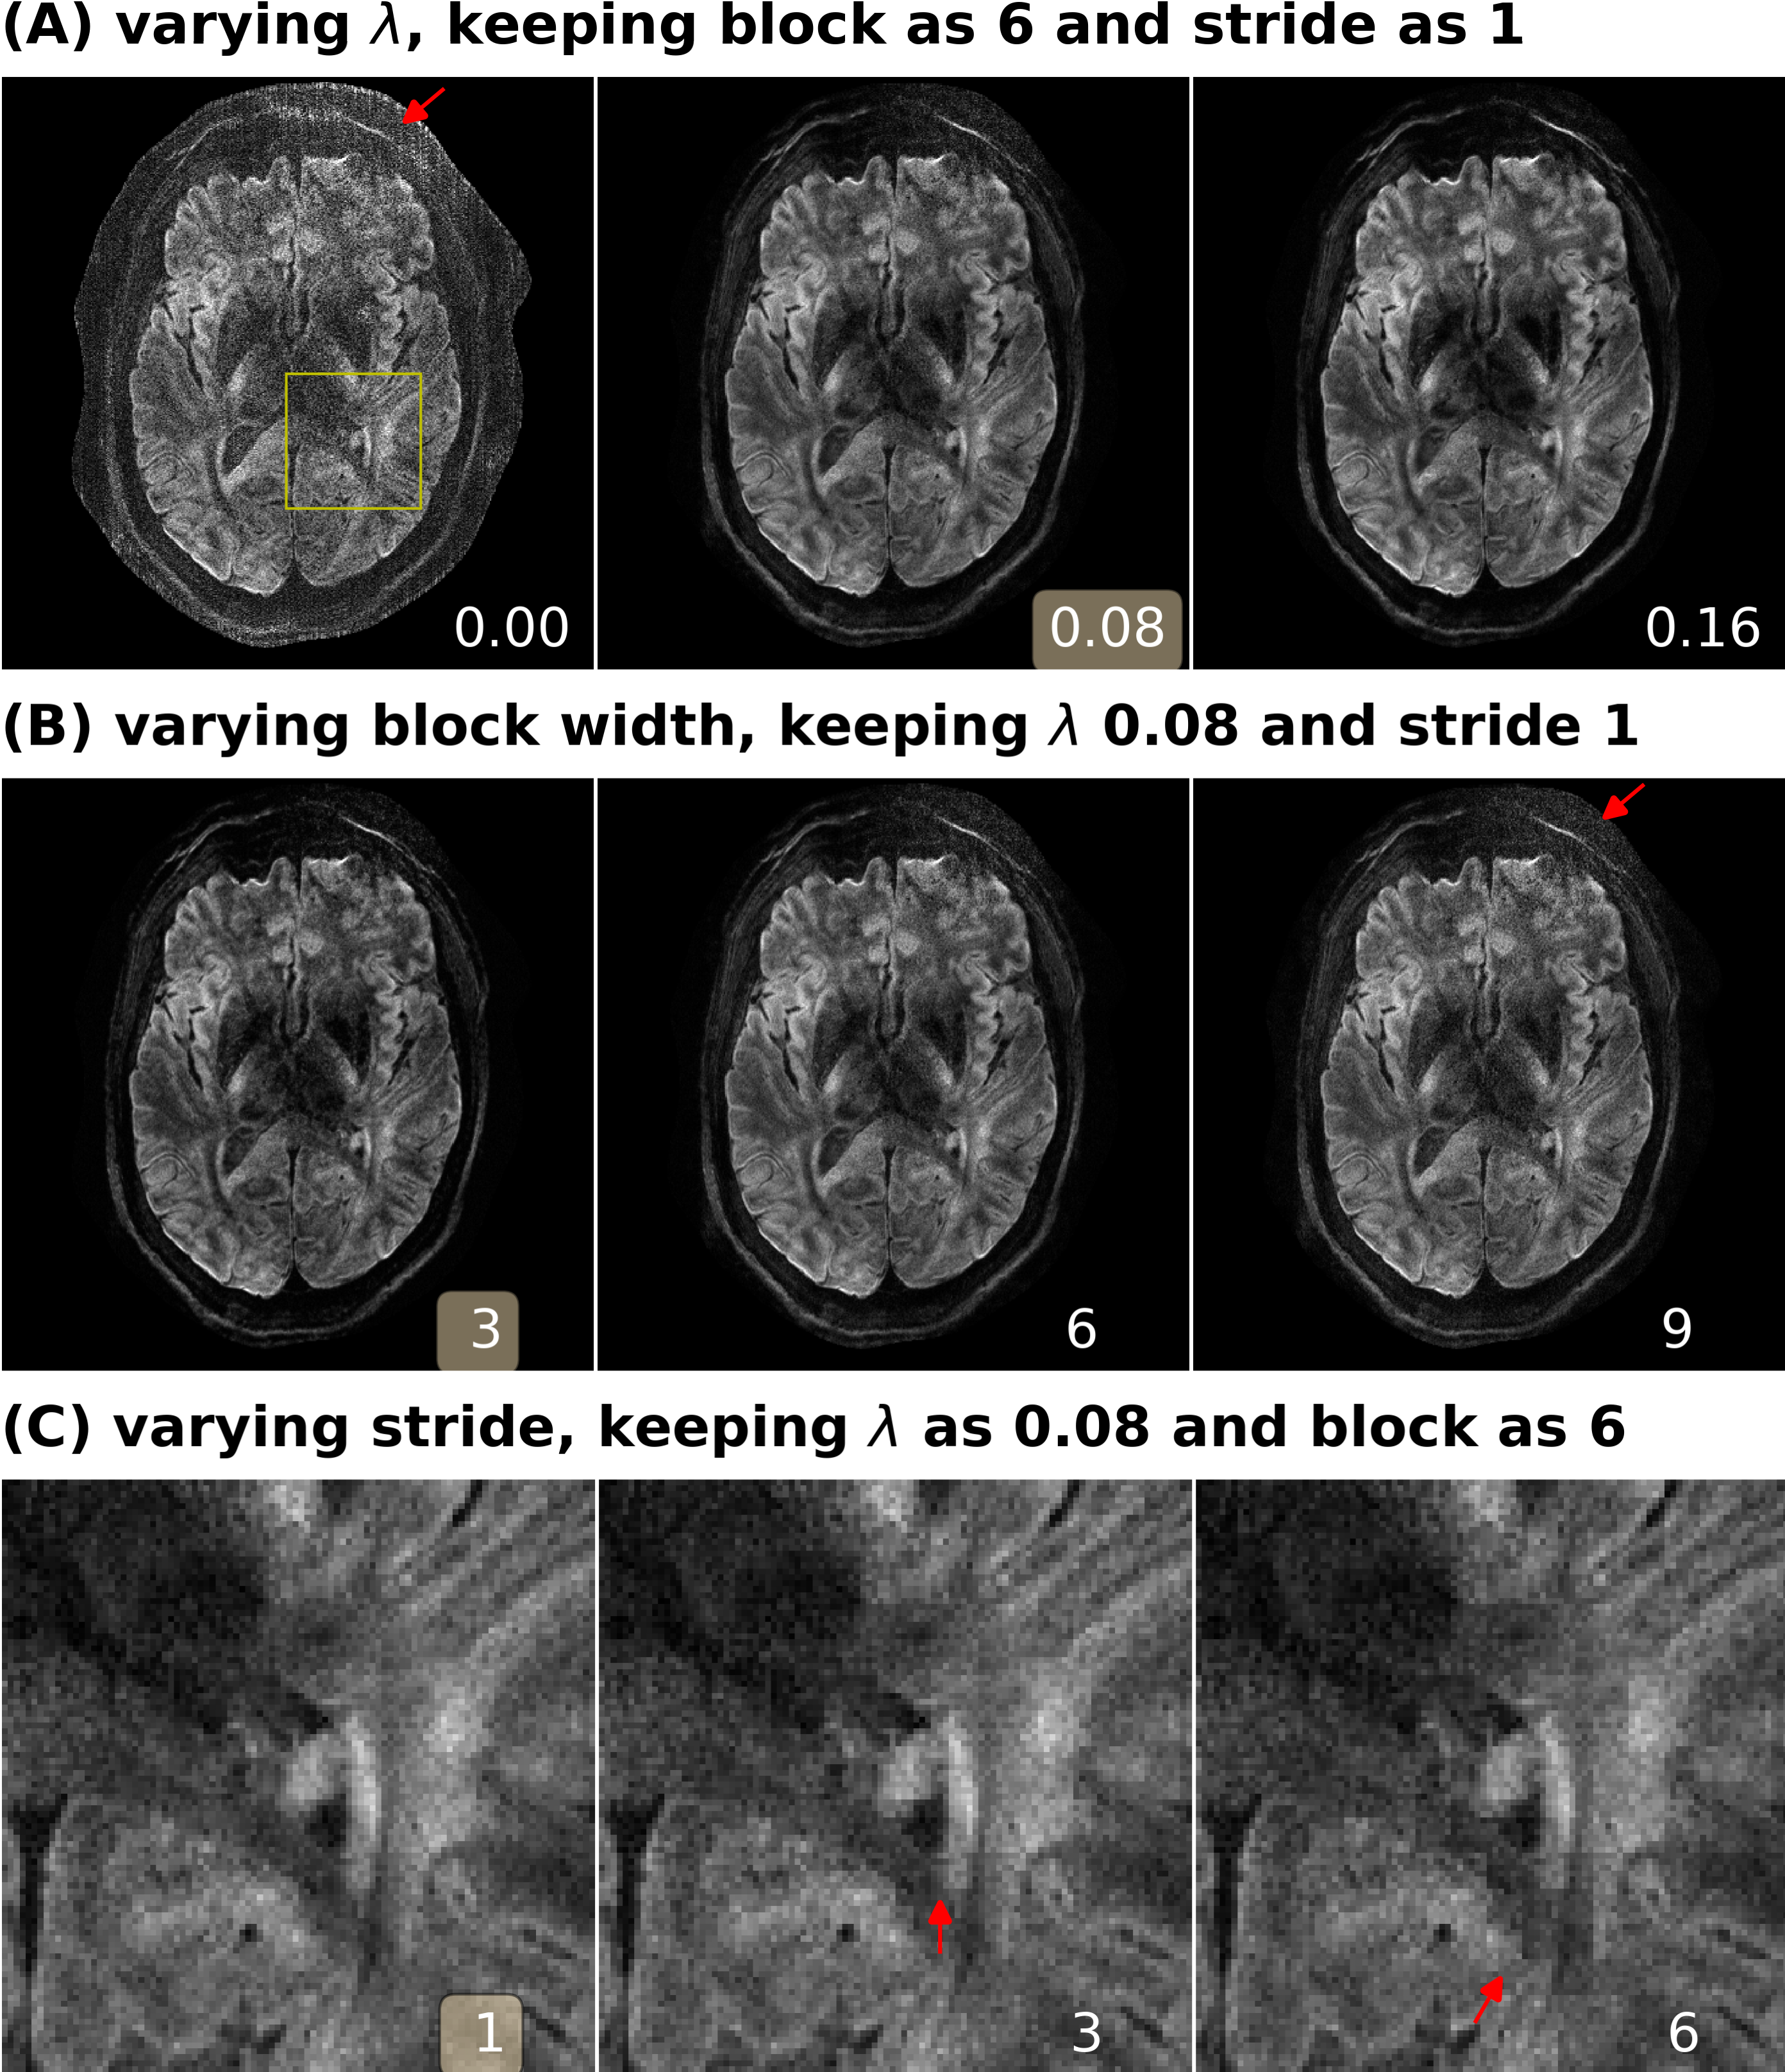
\includegraphics[width=\textwidth]{../figures/fig6.png}
        \caption{Analysis of reconstruction parameters based on
        the 3-scan trace acquisition with $0.5\times0.5\times2.0$~mm$^3$
        (Protocol \#3 in \cref{TAB:ACQ}).
        Displayed are JETS reconstructed single-direction DW images.
        \textbf{(A)} Varying the regularization strength $\lambda$
        from $0$ to $0.08$ and $0.16$.
        \textbf{(B)} Varying \hl{the block width} from $3$ to $6$ and $9$.
        \hl{The red arrow indicates increased noise
        with the large block width.}
        \textbf{(C)} Varying the stride size from $1$ to
        $3$ \hl{(partially overlapping)} and
        $6$ (non-overlapping).
        \hl{The red arrows indicate blocky artifacts.}}
        \label{FIG:ablation}
    \end{figure}

    % ========= %
    \subsection{Analysis of reconstruction parameters}

    Here we provide a systematic analysis of
    the proposed JETS reconstruction
    with LLR regularization applied to
    the spatial-diffusion dimension, as shown in \cref{FIG:ablation}.

    First, we varied the regularization strength $\lambda$.
    We tested values of $0$, $0.08$, and $0.16$.
    The reconstruction with $\lambda = 0$ in \cref{EQU:solve_dwi}
    corresponds to parallel imaging reconstruction
    without LLR regularization.
    It is worth noting that the proposed NAViEPI sequence
    demonstrates high-quality sub-millimeter DW images
    ($0.5\times0.5\times2.0$~\si{\cubic\mm} in this example).
    The DW images can be further improved
    with the use of LLR regularization, i.e., reduced noise,
    as seen in the reconstruction with $\lambda=0.08$.
    Increasing $\lambda$ (e.g.~$0.16$) further reduces noise,
    but at the cost of increased blurring.
    Therefore, $\lambda=0.08$ was selected in this work.

    % TODO: rewrite!!!
    \marginnote{R990.4.a}
    Second, besides the regularization strength,
    the block size (i.e., the area of 2D patches) also
    plays a role in denoising.
    We employed square blocks in this work.
    Here, \hl{the block width} of $3$ shows the best denoising
    as compared to $6$ and $9$,
    especially in the peripheral brain region.

    Third, we varied the stride, i.e.,
    the step from one local patch to the next.
    The use of overlapping LLR
    (\cref{FIG:ablation} (C) left)
    better suppresses blocky artifacts,
    \marginnote{R990.4.b}
    compared to \hl{the partially overlapping (stride $<$ block)} LLR
    (\cref{FIG:ablation} (C) middle)
    and \hl{the non-overlapping (stride $=$ block)} LLR
    (\cref{FIG:ablation} (C) right).

    \begin{figure}
        \centering
        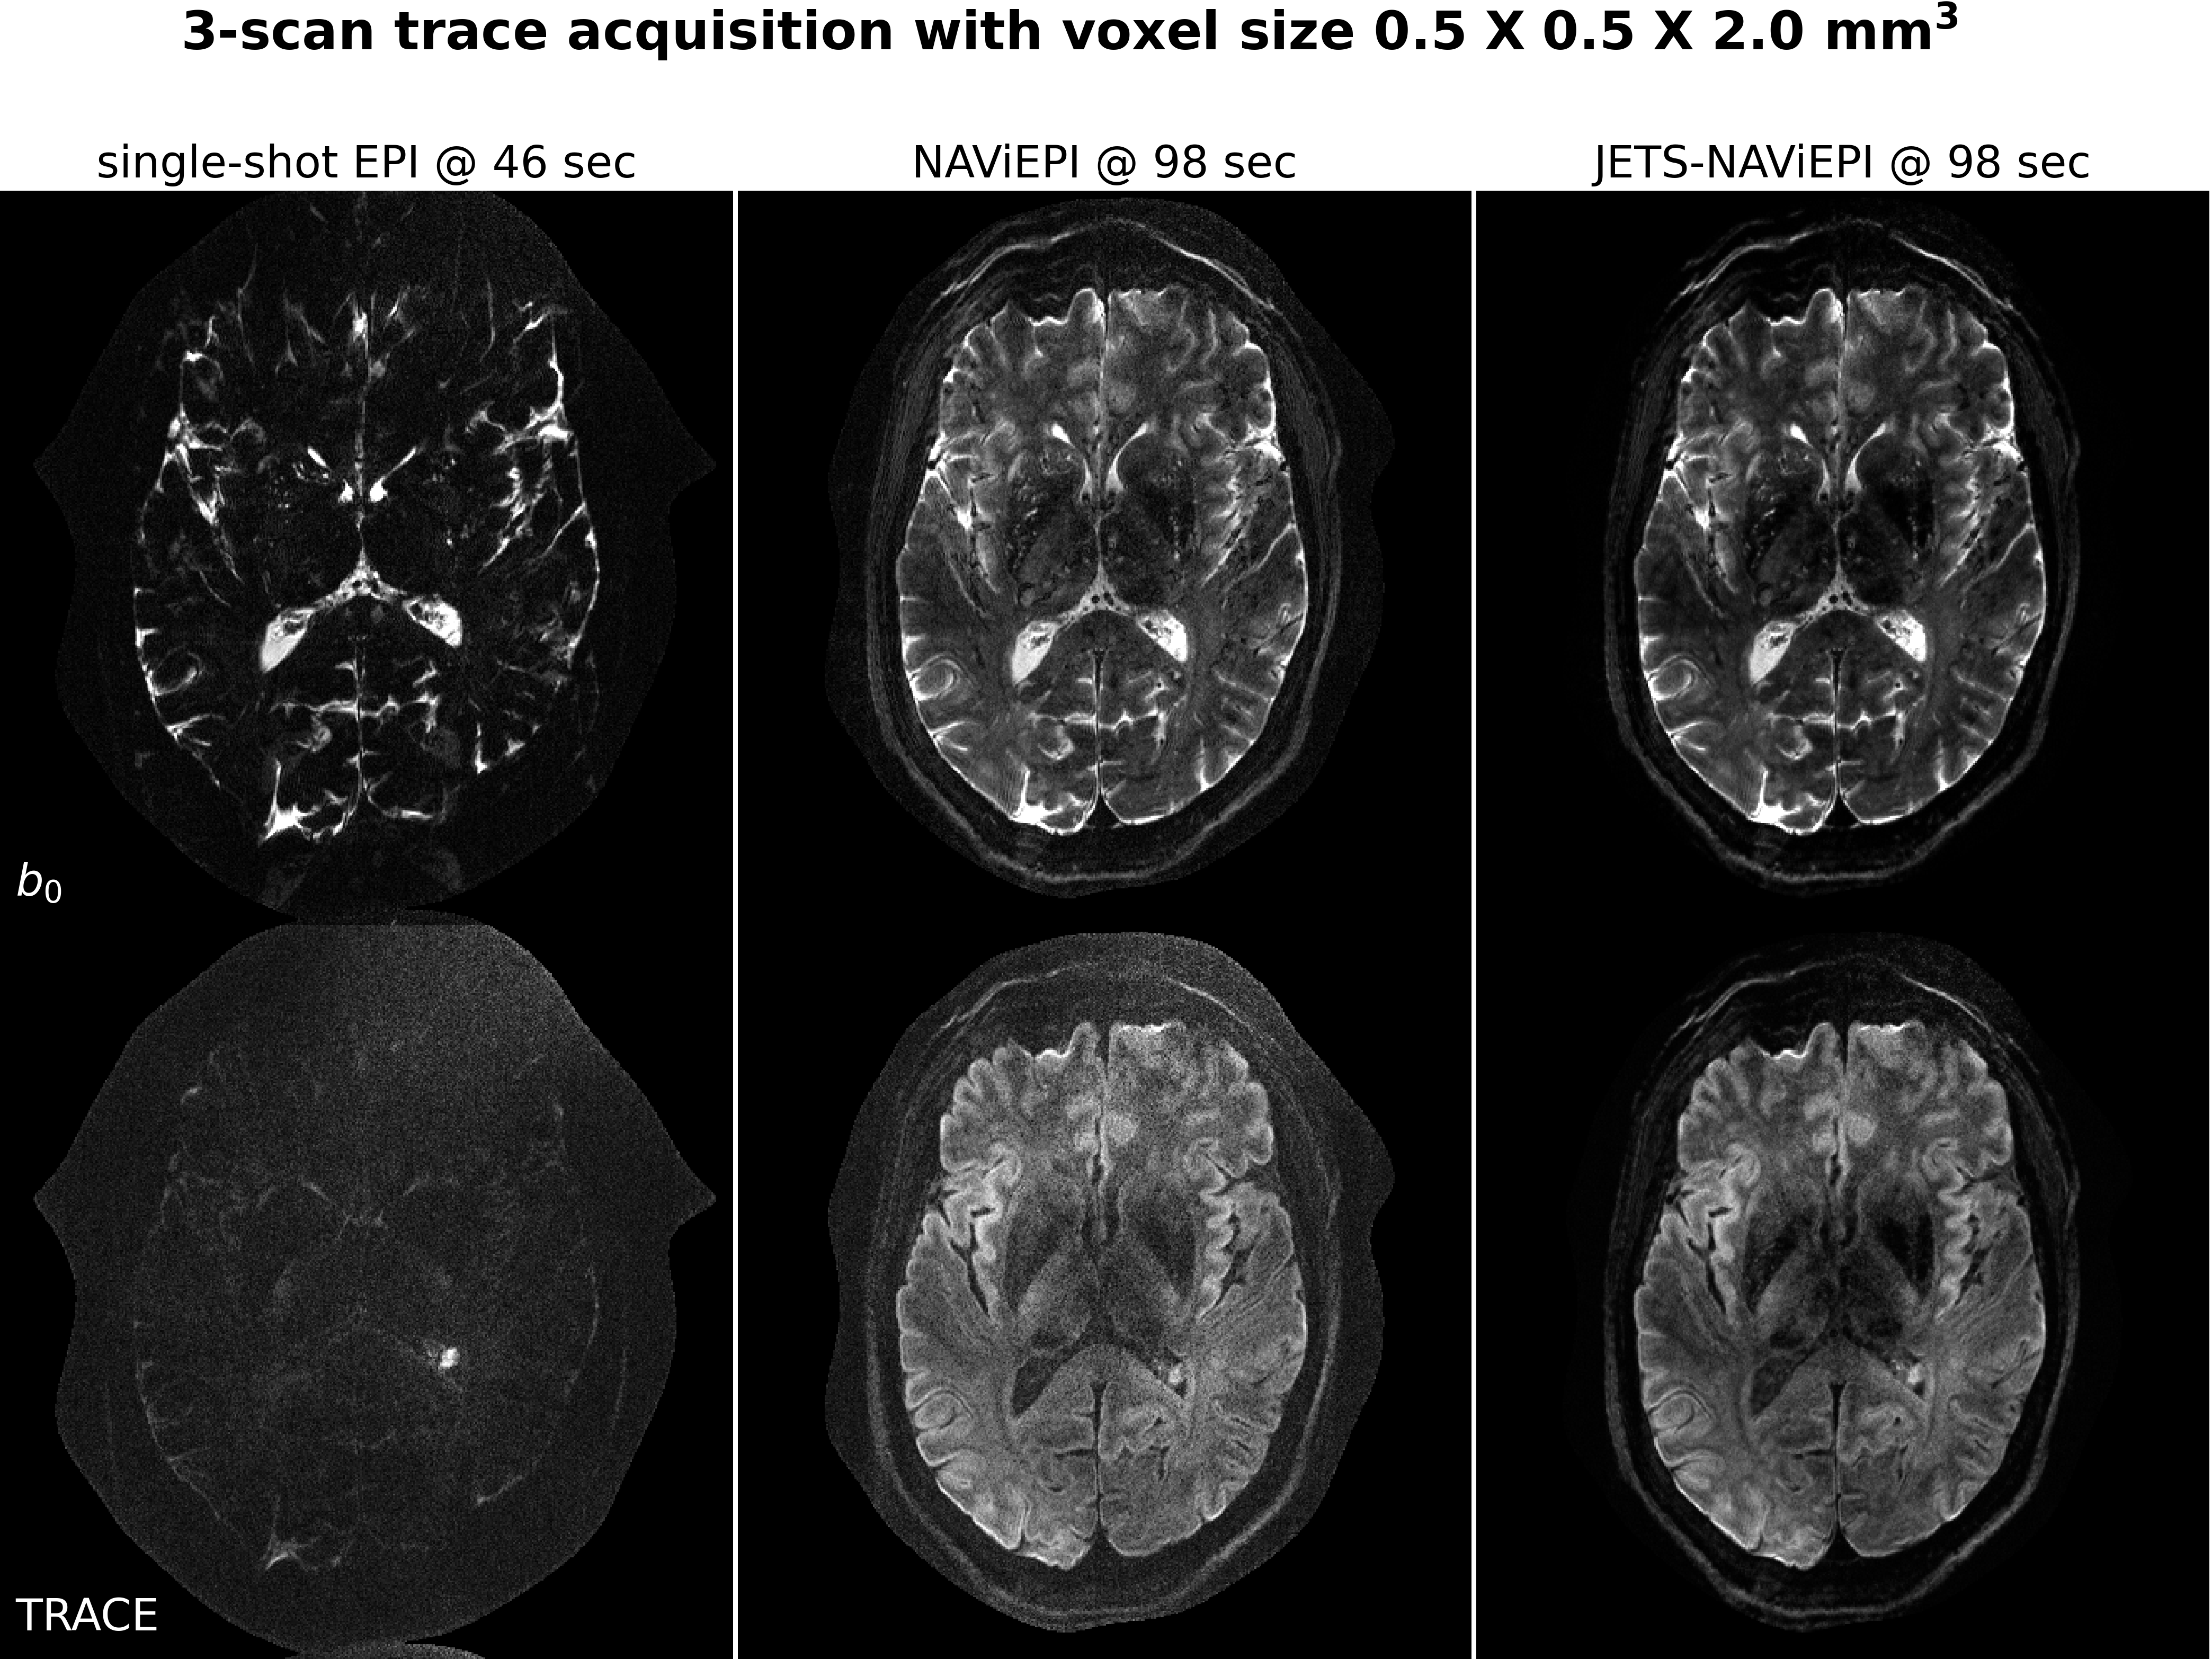
\includegraphics[width=\textwidth]{../figures/fig7.png}
        \caption{Sampling efficiency of the proposed NAViEPI sequence.
        5-shot NAViEPI acquisition with the voxel size
        $0.5\times0.5\times2.0$~mm$^3$ (Protocol \#3)
        was compared with single-shot EPI acquisition (Protocol \#4).
        Both the 1st and the 2nd columns were reconstructed
        via parallel imaging without LLR regularization,
        whereas the 3rd column was reconstructed via JETS.}
        \label{FIG:0.5mm_shots}
    \end{figure}

    % ========= %
    \subsection{Sampling efficiency of NAViEPI}

    As shown in \cref{FIG:0.5mm_shots},
    NAViEPI achieves sub-millimeter resolution
    (voxel size $0.5\times0.5\times2.0$~mm$^3$)
    with the use of a 5-shot acquisition.
    When compared to a single-shot acquisition
    with the same voxel size,
    the acquisition time of NAViEPI is about two times longer,
    but the image quality of NAViEPI is remarkably improved.

    In the sub-millimeter imaging scenario,
    the increased base resolution requires longer TE (\SI{143}{\ms})
    in the single-shot acquisition,
    which results in significant signal loss due to $T_2$ relaxation.
    Therefore, sub-millimeter DWI necessitates multi-shot acquisition,
    which is subject to shot-to-shot phase variation and long scan time.
    However, NAViEPI solves both challenges.
    The 5-shot acquisition reduces TE to \SI{58}{\ms},
    and thus retains SNR significantly
    compared to the single-shot acquisition.
    Moreover, the JETS reconstruction can help to reduce noise
    and improve structural visibility.

    \begin{figure}
        \centering
        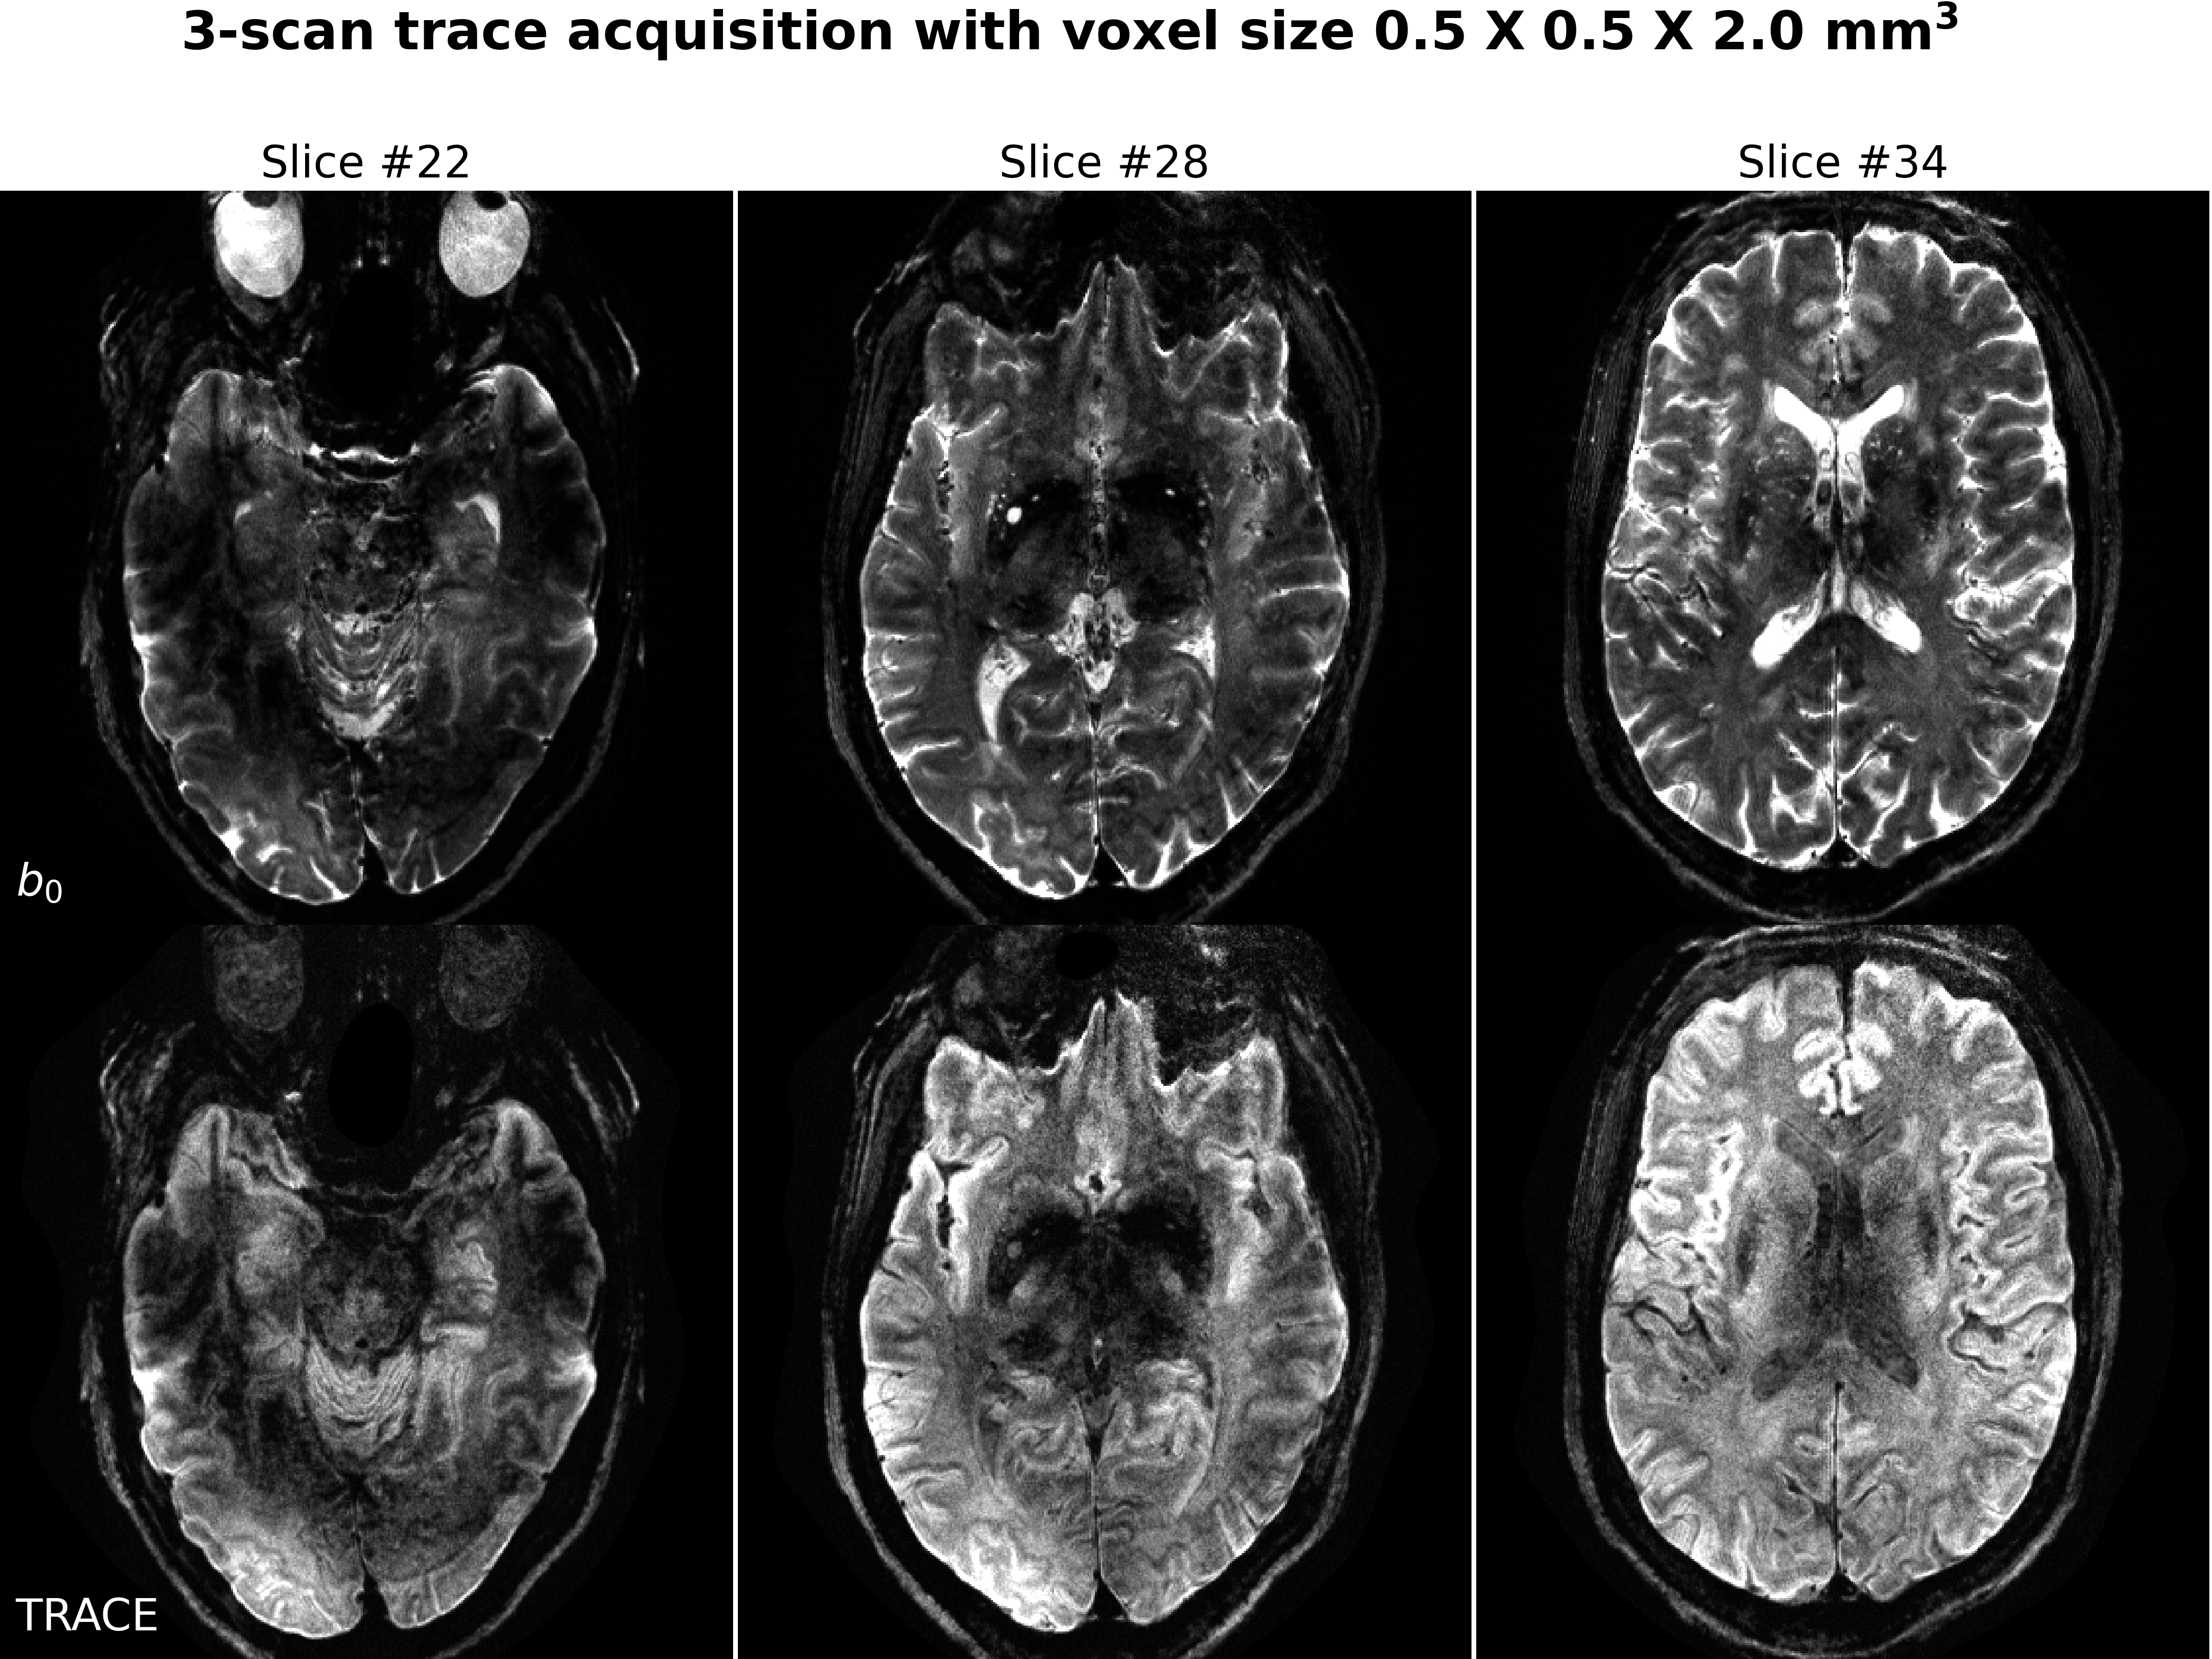
\includegraphics[width=\textwidth]{../figures/fig8.png}
        \caption{Reconstruction of the 3-scan trace acquisition with
        the voxel size $0.5\times0.5\times2.0$~mm$^3$ (Protocol \#3)
        at different slices.}
        \label{FIG:0.5mm_slice}
    \end{figure}

    \cref{FIG:0.5mm_slice} shows the JETS reconstructed $b_0$
    and TRACE images in different slice locations.
    Admittedly, the lower brain region (e.g.~slice \#22)
    exhibits inhomogeneous and lower signal intensity
    than the upper slices.
    Such inhomogeneity can be alleviated with
    the use of multi-channel parallel transmission
    \citep{katscher_2003_ptx,grissom_2010_ptx}.

    \marginnote{R990.7}
    \hl{Here, \mbox{\cref{FIG:ablation,FIG:0.5mm_shots}}
    select a slice with a benign lesion
    (the circular bright spot) within the left ventricle.
    \mbox{\cref{FIG:0.5mm_slice}} displays three representative slices:
    (left) the lower brain region
    which identifies the $B_1^+$ field inhomogeneity,
    (middle) the middle brain slice
    which shows susceptibility artifacts in the frontal region,
    and (right) the upper brain slice which shows the ventricle.}


    \begin{figure}
        \centering
        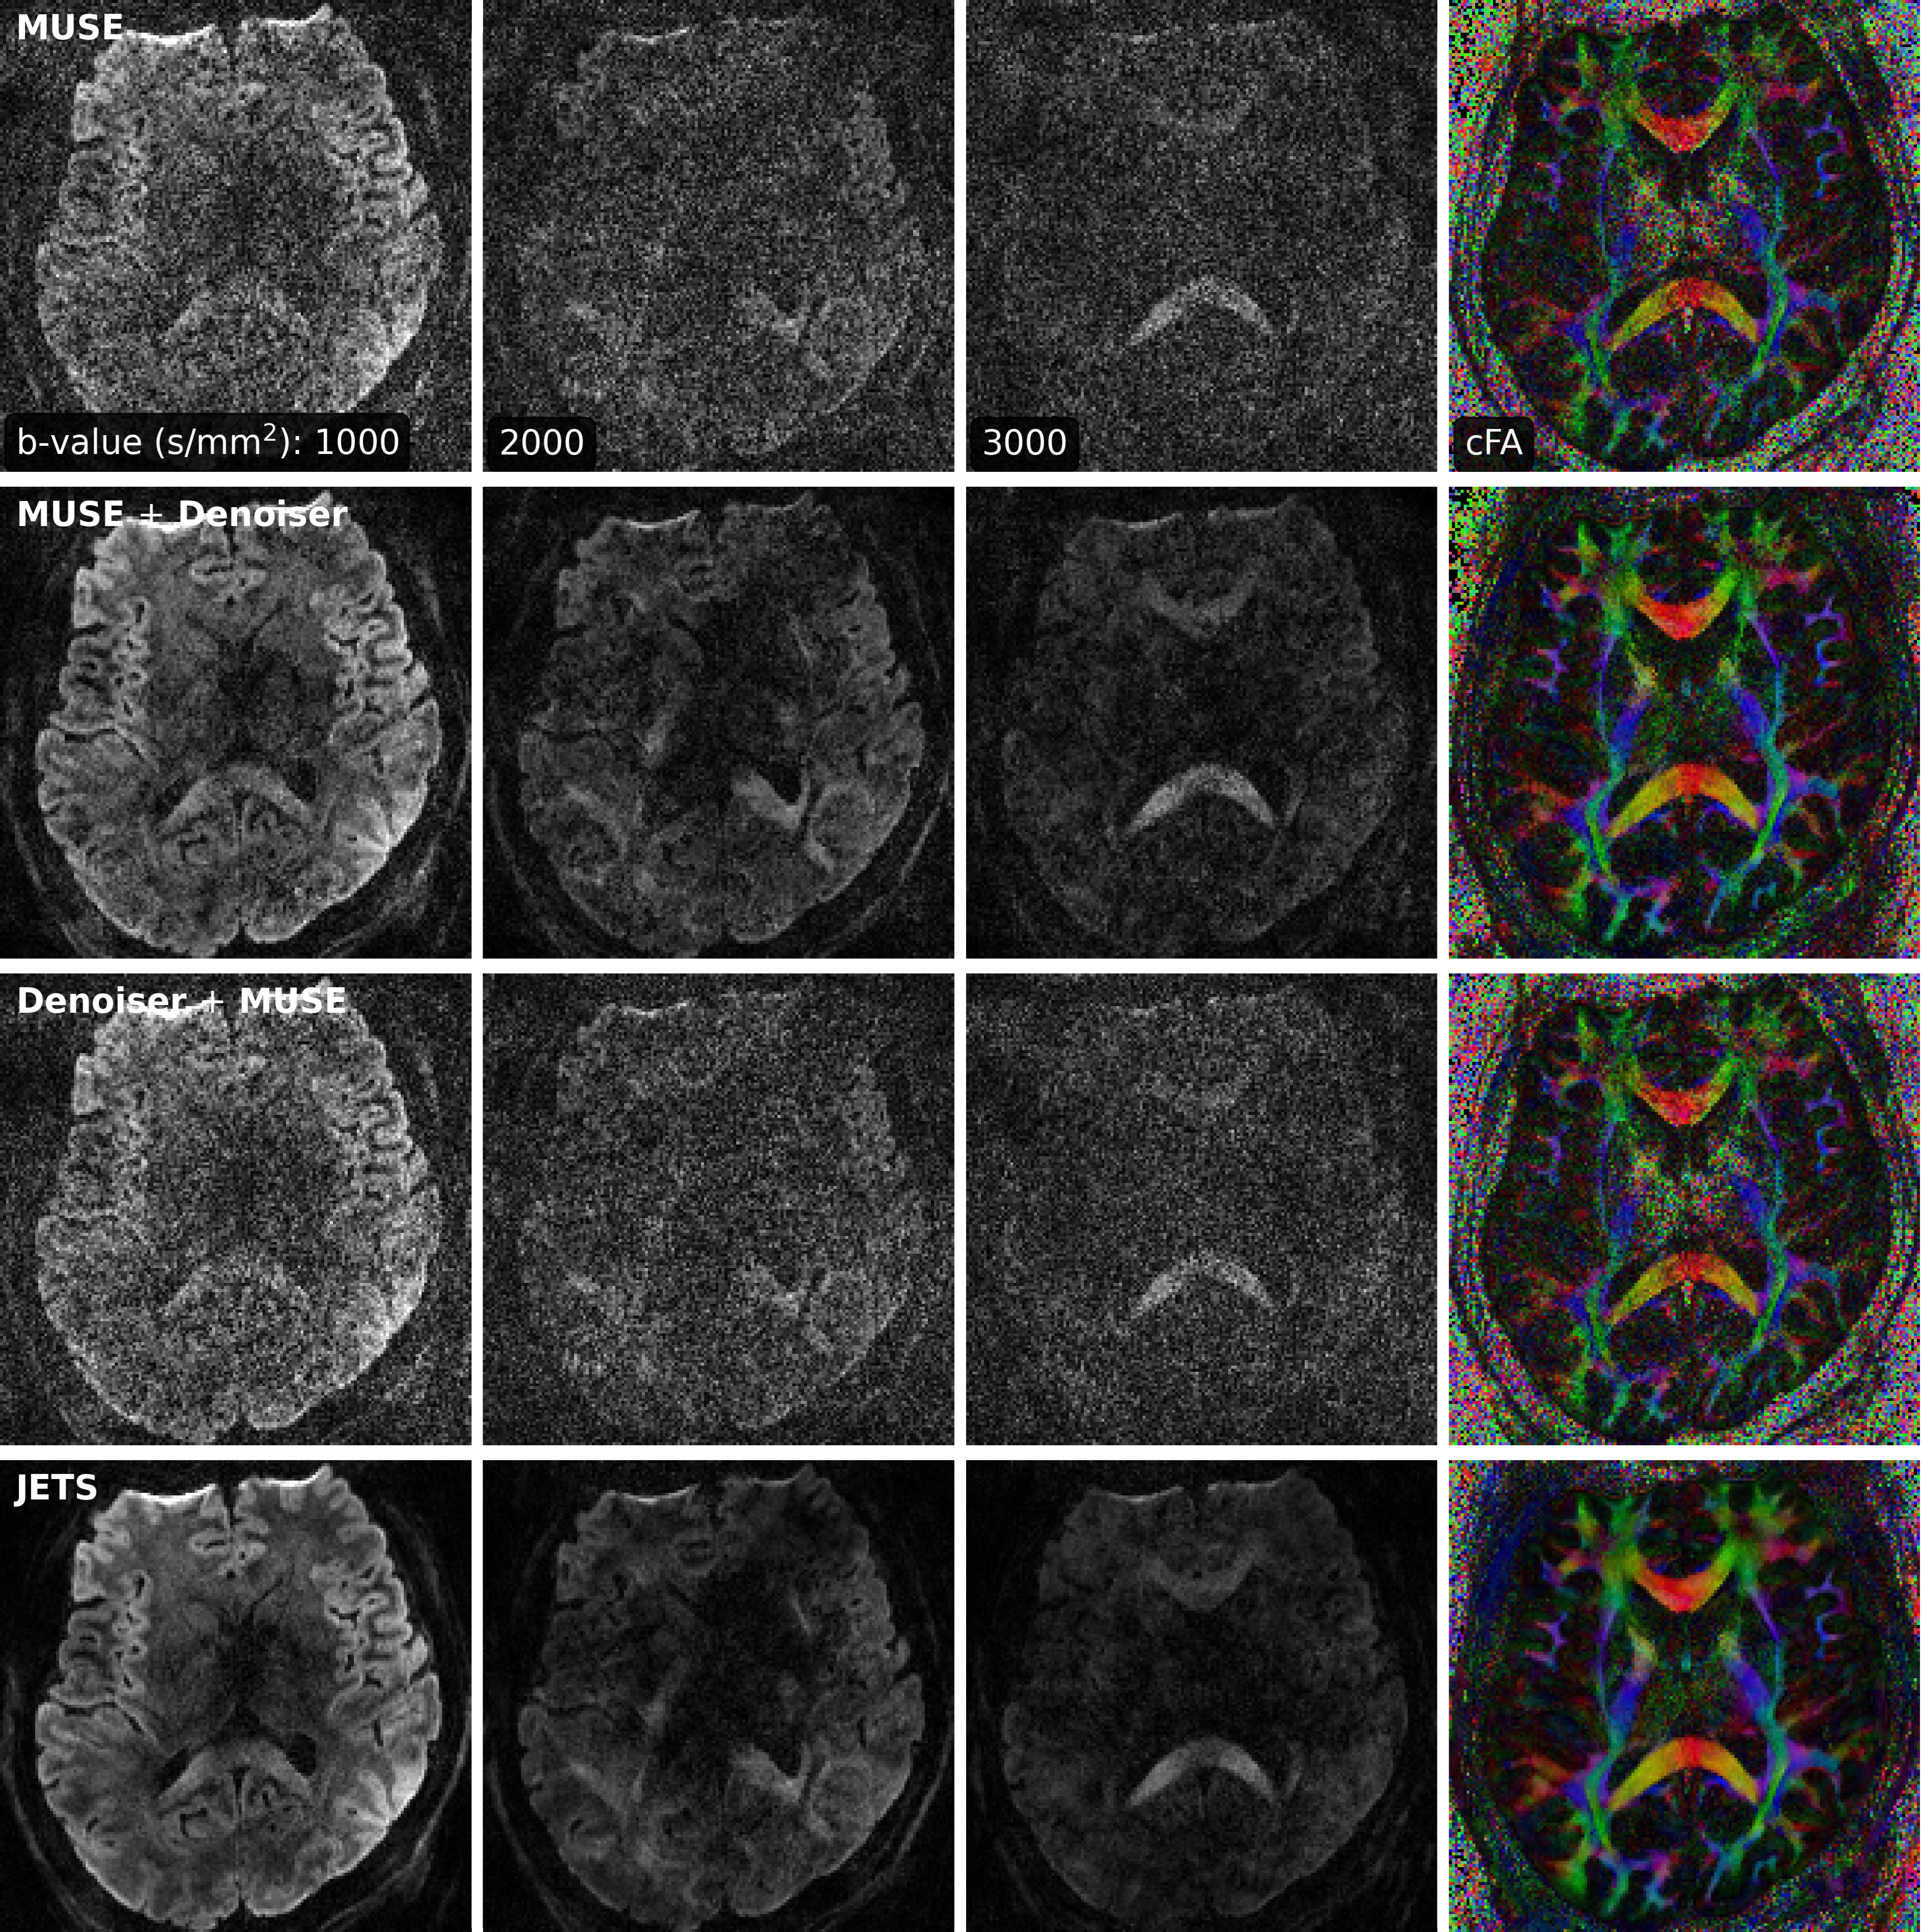
\includegraphics[width=\textwidth]{../figures/fig9.png}
        \caption{Comparison of three-shell DWIs and
        cFA maps with data acquired by Protocol \#2 in \cref{TAB:ACQ}.
        Reconstruction methods from top to bottom were
        MUSE, MUSE with the local-PCA denoiser,
        the application of the denoiser on shot images before the shot combination in MUSE,
        and the proposed JETS method.}
        \label{FIG:1.0mm_dti}
    \end{figure}

    \subsection{Diffusion tensor imaging}

    Protocol \#2 in \cref{TAB:ACQ} yields an acceleration factor of
    $6 \times 3$ per shot, resulting in severe noise amplification
    in MUSE reconstructed DWIs, as shown in \cref{FIG:1.0mm_dti}.
    \marginnote{R990.7}
    \hl{Here, a slice that highlights the corpus callosum is displayed,
    and the diffusion direction at the $b$-value of
    \mbox{\SI{3000}{s/mm^2}} with bright signal
    within the corpus callosum is shown.}
    The local-PCA denoiser substantially removes noise,
    but the DWI at high $b$-values still illustrates more noise,
    compared to the proposed JETS reconstruction.
    \marginnote{R990.3.b.1}
    \hl{On the other hand, we applied the local-PCA denoiser
    before the shot combination in MUSE.
    As shown in \mbox{\cref{FIG:1.0mm_dti}},
    this approach is less effective
    compared to the application of the denoiser after the shot combination,
    because shot images were reconstructed from the central $k$-space region
    and have a coarse resolution.}

    \clearpage

    % ************************************************************************ %
    \section{Discussion}
    \label{SEC:Disc}

    This work reports a novel DW-MRI technique, JETS-NAViEPI.
    NAViEPI (1) achieves the fast and efficient acquisition of
    both imaging and navigator echoes,
    (2) enforces consistent effective ESP between the two echoes, and
    (3) allows for undersampled iEPI as well as a large number of shots.
    Moreover, compared to the single-shot acquisition,
    joint $k$-$q$-slice reconstruction
    with $k_y$-shift encoding on NAViEPI
    retains SNR and reduces aliasing artifacts in DW images.
    As a result, JETS-NAViEPI renders high spatiotemporal resolution
    diffusion MRI protocols in \SI{7}{\tesla},
    e.g., a 3-scan trace acquisition with the voxel size
    $0.5\times0.5\times2.0$~mm$^3$ at \SI{1.5}{\minute}.
    % (FK: This is more or less a repetition of the results section. We should discuss here what the reason for the improved performance is)

    One limitation of JETS-NAViEPI is the long reconstruction time
    due to the simultaneous reconstruction of all DW images and
    the use of overlapping locally low-rank regularization.
    The reconstruction for the Protocol \#3 in \cref{TAB:ACQ}
    on an A100 GPU takes about \SI{2}{\minute} per multi-band slice.
    To reduce the computation time, coil compression algorithms
    \citep{buehrer_2007_scc,huang_2008_scc}
    can be employed to reduce the number of coils for image reconstruction.
    Moreover, one can deploy multi-GPU distributed computing
    or modern optimization algorithms
    (e.g.~stochastic gradient descent) \citep{ong_2020_extreme}
    to speed up the reconstruction.

    Neither the signal modeling in
    \cref{EQU:model_shot,EQU:model_dwi}
    nor the LLR regularization considers the subject motion.
    In the presence of motion, the regularized reconstruction can degrade.
    To overcome this problem, scout-informed motion estimation
    and reconstruction \citep{polak_2022_samer}
    could be integrated into the framework.

    Another potential extension of this work is
    to incorporate distortion correction.
    The standard distortion correction method is
    known as TOPUP \citep{andersson_2003_topup},
    which acquires two scans
    with opposing phase-encoding directions to
    obtain the field inhomogeneity map and
    then performs conjugate phase reconstruction
    to correct for distortion.
    \marginnote{R989.4, R990.13}
    Alternatively, \hl{a} multi-echo acquisition could be used
    for the coil sensitivity reference scan, such that
    both coil sensitivity and $B_0$ field inhomogeneity maps
    could be reconstructed from the data.

    This work employed a single regularization weight $\lambda$
    to enforce low rankness along the spatial-diffusion direction.
    However, SNR may be heterogeneous within the FOV.
    Therefore, one single regularization scalar may be inadequate
    to cover the whole FOV.
    Beyond this SVT-based reconstruction,
    one can seek to use machine learning to
    learn a $q$-space prior as the regularizer
    \citep{hammernik_2018_varnet,lam_2019_mrsi,mani_2021_qmodel}.

    Although NAViEPI employs navigators for
    the acquisition of shot-to-shot phase variation,
    it is worth noting that phase behavior depends on
    several hard-to-control factors
    such as pulsatile motion, bulk motion,
    locations within the brain, and
    diffusion sensitization strength.
    Therefore, more comprehensive modeling or post-processing
    such as image registration can be considered in future work.

    This work compared LLR regularized JETS to
    MUSE post-processed by the local PCA denoiser
    \citep{cordero_2019_cplxdwi}.
    \marginnote{R990.3.b.2}
    \hl{Both the LLR regularization and the local PCA denoiser
    are based on the principle that low rankness exists
    in the spatial-diffusion dimension,
    where the spatial content is extracted from local patches
    within the full image volume
    and the diffusion dimension is from the $q$-space encoding.
    Both of them demonstrate effective denoising capabilities
    and allow for high-quality DW-MRI image reconstruction
    from the accelerated acquisition.}

    Technically, the LLR regularization is realized
    by soft thresholding of the singular values
    of the spatial-diffusion matrices, whereas
    the denoiser performs hard thresholding.
    Both approaches demonstrate effective noise removal.
    In the scenario of accelerated acquisitions,
    one can employ both approaches to maximally boost SNR,
    i.e., the use of LLR regularization for image reconstruction
    followed by the denoiser as a post-processing step.

    While this work reconstructs all DW images and
    then performs model fitting,
    an alternative approach is to directly estimate
    $b_0$ and diffusion tensors
    from measured $k$-$q$-space data
    using model-based reconstruction
    \citep{knoll_2015_mobadiff,dong_2018_mobadiff,shafieizargar_2023_adept}.
    Compared to DW image reconstruction,
    model-based reconstruction solves for a fewer number of unknowns,
    but requires strict diffusion tensor modeling
    and the use of nonlinear least square solvers.

    % ************************************************************************ %
    \section{Conclusions}
    \label{SEC:Conc}

    We demonstrated the JETS-NAViEPI technique, which integrates
    a $k_y$-shifted encoding navigator-based interleaved EPI sequence
    and joint reconstruction with overlapping locally low-rank regularization
    for high spatial-angular-temporal resolution DW-MRI at \SI{7}{\tesla}.
    This technique allows for high-quality DW image reconstruction
    with accelerated acquisitions.

    % ************************************************************************ %
    \section*{Funding}

    Funding by the German Research Foundation (DFG)
    is gratefully acknowledged
    (projects 513220538, 512819079;
    and project 500888779 of the RU5534 MR biosignatures at UHF).
    In addition, funding by the National Institutes of Health (NIH),
    R01 EB024532 and P41 EB017183, is gratefully acknowledged.

    % https://hpc.fau.de/faqs/#innerID-1437
    In addition, we gratefully acknowledge the scientific support and HPC resources
    provided by the Erlangen National High Performance Computing Center (NHR@FAU)
    of Friedrich-Alexander-University Erlangen-Nuremberg (FAU)
    under the NHR project b143dc.
    NHR funding is provided by federal and Bavarian state authorities.
    NHR@FAU hardware is partially funded by the German Research Foundation (DFG) -- 440719683.

    % ************************************************************************ %
    \section*{Data and code available statement}

    In the spirit of reproducible and open science,
    we publish our source code
    (\url{https://github.com/ZhengguoTan/sigpy})
    as well as the raw $k$-space data
    (\url{https://doi.org/10.5281/zenodo.7548595}).
    We also provide interactive demonstrations
    of the reconstruction procedure
    (\url{https://github.com/ZhengguoTan/demo_jets_diffusion_mri_7t}).

    % ************************************************************************ %
    \section*{Acknowledgments}

    The authors thank Dr.~Peter Neher for the discussion on MITK-Diffusion.
    The authors thank
    Dr.~Berkin Bilgic for making the MUSSELS source code
    (\url{https://bit.ly/2QgBg9U}) publically available,
    Dr.~Erpeng Dai for sharing the JULEP source code
    (\url{https://github.com/daiep/JULEP}) on GitHub,
    and Dr.~Zhiyong Zhang for sharing the SPA-LLR source code
    (\url{https://github.com/ZZgroupSJTU/PMCmsDTI}) on GitHub.
    The authors also thank Dr.~Philipp Ehses for the discussion on
    twixtools (\url{https://github.com/pehses/twixtools}).

    \bibliographystyle{elsarticle-harv}  % unsrt
    \bibliography{ref}

\end{document}
